\chapter{Basic Simplification Algorithm}
\thispagestyle{empty}% no page number in chapter title page
In this section is presented a basic algorithm for mesh simplification. The algorithm is founded on several components: iterative vertex contraction and quadric error metric. This part elaborates basics of one of the most popular methods for mesh simplification created by Michael Garland.
\numberwithin{equation}{section}
\section{Motivation}
The core of the algorithm is based on Michael Garland's work Quadric-Based Polygonal Surface Simplification \cite{garland99}, where he suggests an algorithm capable of producing high-quality approximations of polygonal meshes. The main assumption is that the approximation need not to maintain the topology of the original surface and is a nicely balanced trade-off between quality and size.

The goal of this work was to adopt this algorithm to a parallel framework with adaptive thresholding, capable of fast progresive mesh streaming \cite{yang01} for renderer engines in browsers. An example of such a renderer is IndoorViewer product created by NavVis. Depending on selected mesh resolution and level of details an appropriate mesh will be streamed to a browser. Therefore, the size and quality is crucial for the endpoint users to get maximal usability. Using the assumption that planar surfaces need much less triangles to describe geometry, while preserving details at non-planar surface. Light and detailed meshes can be generated which are suitable for streaming purposes.
\clearpage

\section{Iterative Vertex Contraction}
The simplification algorithm is based on several atomic operations. The most important of them is an edge contraction. A pair of contraction is defined as $(\mathbf{v_i}, \mathbf{v_j})\rightarrow\bar{\mathbf{v}}$. The atomic operation of a contraction is then defined as:

\begin{enumerate}
\item Move the vertices $\mathbf{v_i}$ and $\mathbf{v_j}$ to the position $\bar{\mathbf{v}}$
\item Replace all connections of $\mathbf{v_j}$ with $\mathbf{v_i}$
\item Remove $\mathbf{v_j}$ and all faces which belong both to $\mathbf{v_i}$ and $\mathbf{v_j}$. In Figure~\ref{fig:edge_contraction_ref} the gray faces.
\end{enumerate}

\begin{figure}[h!]
  \begin{center}
    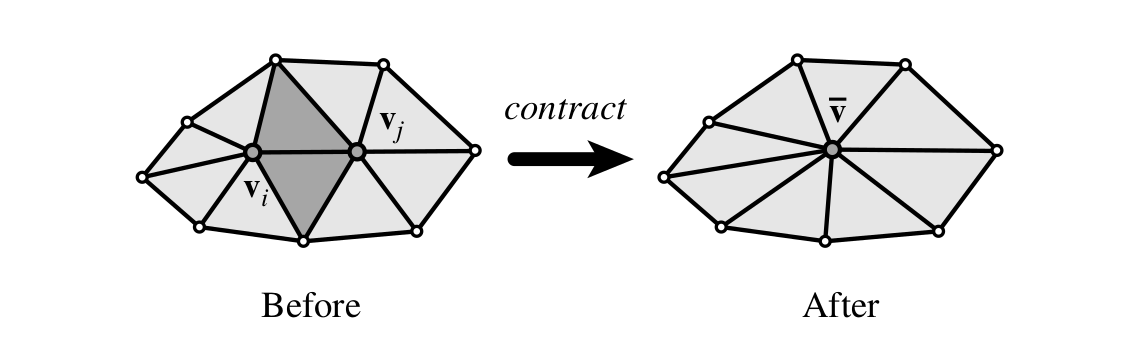
\includegraphics[width=14cm]{edge_contraction}
    \caption{Contraction of an edge. Remove $\mathbf{v_j}$ and move remaining edges to $\mathbf{v_i}$ \cite{garland99}.}
    \label{fig:edge_contraction_ref}
  \end{center}
\end{figure}

The mentioned algorithm is a greedy procedure driven by the cost of contraction \cite{cormen01}. It stops when the current threshold level is reached. To achieve simplification we apply a sequence of edge contraction. Where the sequence is created as follows \cite{garland97}:

\begin{enumerate}
\item Select a set of candidate vertex pairs.
\item Assign a cost of contraction to each candidate.
\item Place all candidates in a heap keyed on cost with the minimum cost pair at the top.
\item Repeat until the desired approximation is reached:
\begin{enumerate}
\item Remove the pair $(\mathbf{v_i}, \mathbf{v_j})$ of least cost from the heap.
\item Contract this pair.
\item Update costs of all candidate pairs involving $\mathbf{v_i}$.
\end{enumerate}
\end{enumerate}

Each edge is associated with a cost of contraction, which is basically the amount of error made during deletion of a given pair of vertices. This cost is a key in the minimum heap \cite{cormen01} which is iteratively $pop()$. In each main iteration (steps from 1 to 4) we contract edges up to the current adaptive threshold level. If a current edge's cost is bigger or equal than the acceptable error, the main iteration procedure is stopped and the remaining edges in the heap are ignored. In a next iteration, the heap is rebuilt and the error level is slightly increased in such a way that previously contracted regions are even more simplified. The error calculations are based on a hyper-parameters $aggressiveness$ and a current iteration value:
\begin{align}
error(i)=10^{-9}\cdot(i+3)^a
\label{error_formula}
\end{align}
where $i$ is the iteration and $a$ is the aggressiveness.

The formula \ref{error_formula} is inspired by a Github implementation of Fast-Quadric-Mesh-Simplification, where the author introduced adaptive thresholding using \ref{error_formula}. The $aggressiveness$ has to be changed once the different attributes for the error metric are used. The best results for geometry gives value $a=3$ and for the rest of attributes $a=5$ is used.

Rebuilding heap captures the change of geometry made in a contraction for the whole mesh. After one contraction we update only first order neighbors of a given vertex. Therefore, we need to rebuild heap to reflect the global change.

\section{Assessing Cost of Contraction}
This section elaborates the way how to measure the cost of contraction for an edge. For simplicity, the analysis is made just for geometry attributes. Maintaining high level of details and faithful representation of the original mesh, the cost should be reflected in the effect of changing geometry of the surface. Meaning, if the error is small, the geometry changes insignificantly. An edge with a small error is a good candidate for removal.

Because the metric is plane-based, the standard representation of a plane is defined as $\mathbf{n}^T\mathbf{v}+d=0$ with normal  $\mathbf{n} = [a\;b\;c]^T$, $d$ is a scalar constant and $\mathbf{v} = [x\;y\;z]^T$ is a point in $3D$ space. From this, the quadric error metric can formulate as following \cite{garland99}:
\begin{align}
D^2(\mathbf{v}) = (\mathbf{n}^T\mathbf{v}+d)^2 = (ax + by + cz + d)^2
\label{quadric_distance}
\end{align}
The error for the set of planes associated with the vertex $v$ is then defined as (we have to remember that this set is purely conceptual):
\begin{align}
\sum_{i} D_i^2(\mathbf{v}) = \sum_{i} (\mathbf{n_i}^T\mathbf{v}+d_i)^2
\end{align}
Each vertex has an accumulated error metric value for surrounding faces which represents the maximum squared distance to the intersection of all planes spanned by each face.

Figure~\ref{fig:measuring_contraction_ref} shows how removing a pair of contraction $(\mathbf{v}_i, \mathbf{v}_j)$ could look in practice in the $2D$ case. Vertices $\mathbf{v}_i, \mathbf{v}_j$ define set of lines $P_i = \{A,C\}$ and $P_j = \{B, C\}$. The error on each of those vertices equals $E_{plane}(v_i) = E_{plane}(v_j) = 0$ since they both lie on the lines span by thier sets. Let me define a new set which is a union of $ \bar{P} = P_i \cup P_j = \{ A,B,C \}$. Position of $\bar{\mathbf{v}}$ minimizes the sum of square distances the the lines in $\bar{P}$ \cite{garland99}.

\begin{figure}[H]
  \begin{center}
    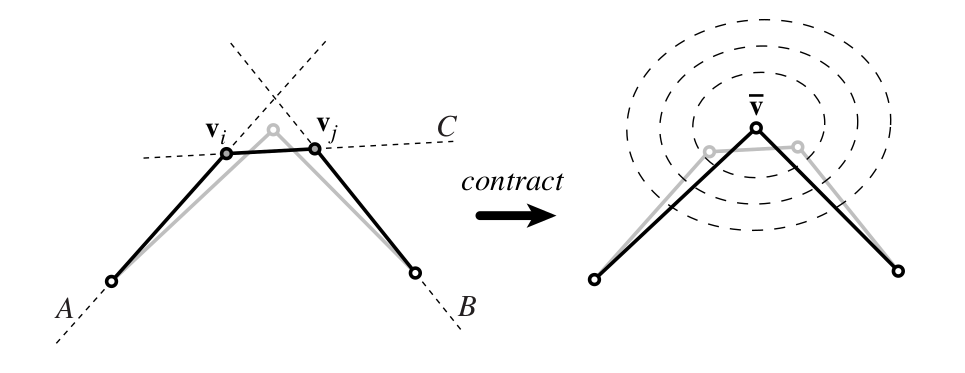
\includegraphics[width=15cm]{measuring_contraction}
    \caption{Measuring contraction cost in 2D where $\bar{\mathbf{v}}$ is a global minimum of our optimization objective. The dotted circles represent iso-lines of the funciton error \cite{garland99}.}
    \label{fig:measuring_contraction_ref}
  \end{center}
\end{figure}

\section{Quadric Error Metric}

In this section the compact representation of the quadric error is introduced. First, previously declared formula of quadric distance is expanded to: $D^2(\mathbf{v})$~\ref{quadric_distance}.
\begin{align}
D^2(\mathbf{v})&=(\mathbf{n}^T\mathbf{v}+d)^2\\
	  &=(\mathbf{n}^T\mathbf{v}+d)(\mathbf{n}^T\mathbf{v}+d)\\
	  &=(\mathbf{v}^T\mathbf{n}\mathbf{n}^T\mathbf{v}+2d\mathbf{n}^T\mathbf{v}+d^2)\\
	  &=(\mathbf{v}^T(\mathbf{n}\mathbf{n}^T)\mathbf{v}+2(d\mathbf{n})^T\mathbf{v}+d^2)
	  \label{quadric_equation}
\end{align}
where $\mathbf{n}\mathbf{n}^T$ is the outer product of the face normal:
\begin{align}
\left[
\begin{array}{rrrr}
a^2 & ab & ac   \\
ab  & b^2 & bc  \\
ac  & bc  & c^2 \\
\end{array}\right]
\end{align}
Therefore, the $quadric\;Q$ is defined as a triple:
\begin{align}
Q = (\mathbf{A},\mathbf{b},c)
\end{align}
Where $\mathbf{A}$ is a $3x3$ matrix, $\mathbf{b}$ is a 3-vector and c is a scalar. Therefore, the equation \ref{quadric_equation} is rewritten to:
\begin{align}
Q(\mathbf{v}) = \mathbf{v}^T\mathbf{A}\mathbf{v} + 2\mathbf{b}^T\mathbf{v} + c
\end{align}
Quadrics provide an intuitive addition operation which is component-wise: $Q_i(\mathbf{v}) + Q_j(\mathbf{v}) = (Q_i + Q_j)(\mathbf{v})$ where $Q_i(\mathbf{v}) + Q_j(\mathbf{v}) = (\mathbf{A_i} + \mathbf{A_j}, \mathbf{b_i} + \mathbf{b_j}, c_i + c_j)$. Using this fact, a single quadric $E_Q$ can easily be defined for the set of planes of a given vertex \cite{garland99} as sum over quadrics for each face:
\begin{align}
E_Q(\mathbf{v}) = \sum_{i} D_i^2(\mathbf{v}) = \sum_{i} Q_i(\mathbf{v}) = Q(\mathbf{v})
\end{align}
In other words, each vertex contains accumulated information about the error for the whole local neighborhood of $\mathbf{v}$. For the pair of vertices the cost of contraction $(\mathbf{v_i}, \mathbf{v_j})\rightarrow\bar{\mathbf{v}}$ is simply:
\begin{align}
Q(\mathbf{\bar{v}}) = Q_i(\mathbf{\bar{v}}) + Q_j(\mathbf{\bar{v}})
\end{align}
The value of $Q(\mathbf{\bar{v}})$ is a key in the min-heap. Tables~\ref{tab:approx_bunny_ref} and~\ref{tab:wireframe_ref} show an example of simplification using quadric metric. Due to complexity of the original Stanford Bunny mesh which has 69451 faces, it was first simplified to 3642 faces and then used as a reference model.

\begin{table}[h!]
\centering
\begin{tabular}{ |c|c| } 
 \hline
 Number of faces & Size in \% of the original mesh\\
 \hline
 3642 faces & 94.7\% \\ 
 2228 faces & 96.8\% \\ 
 1842 faces & 97.3\%\\ 
 1152 faces & 98.3\%\\ 
 665 faces & 99.0\%\\ 
 130 faces & 99.8\%\\
 \hline
\end{tabular}
\caption{Percentage of simplification of the original Stanford Bunny with 69351 faces.}
\end{table}
Table~\ref{tab:original_ref} shows the quality of progressive simplification. 70\% of reduction is hard to distinguish from the original mesh, even the 95\% is still a good approximation and features of the bunny are preserved fairly well.

\begin{center}
  	\begin{table}[H]
  	\begin{center}
  	\begin{tabular}{cc}
	\begin{subfigure}{0.7\textwidth}\centering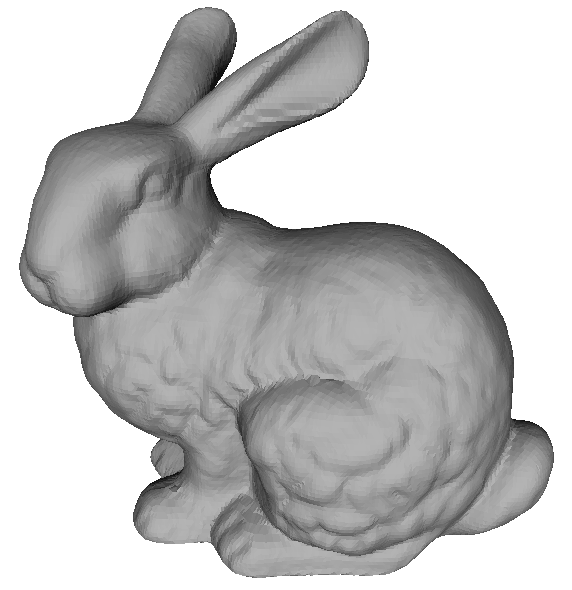
\includegraphics
		[width=0.5\columnwidth]{original_100}\caption{Faces 69451 (100\%)}\label{original_100_ref}\end{subfigure}\\
	\begin{subfigure}{0.7\textwidth}\centering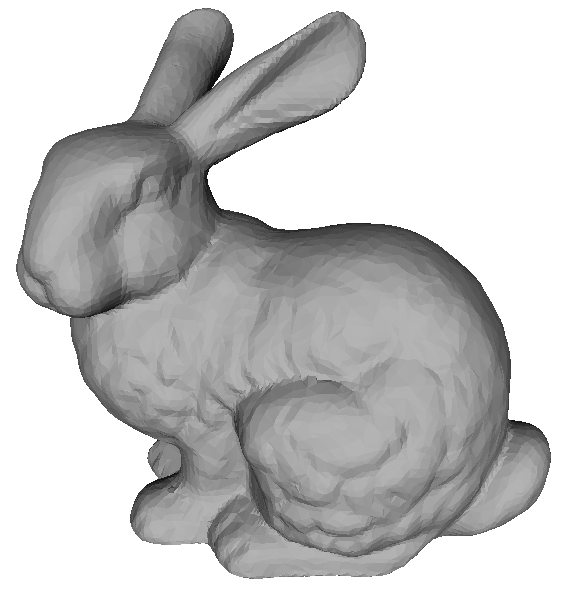
\includegraphics
		[width=0.5\columnwidth]{original_70}\caption{Faces 18892 (30\%)}\label{original_70_ref}\end{subfigure}\\
	\begin{subfigure}{0.7\textwidth}\centering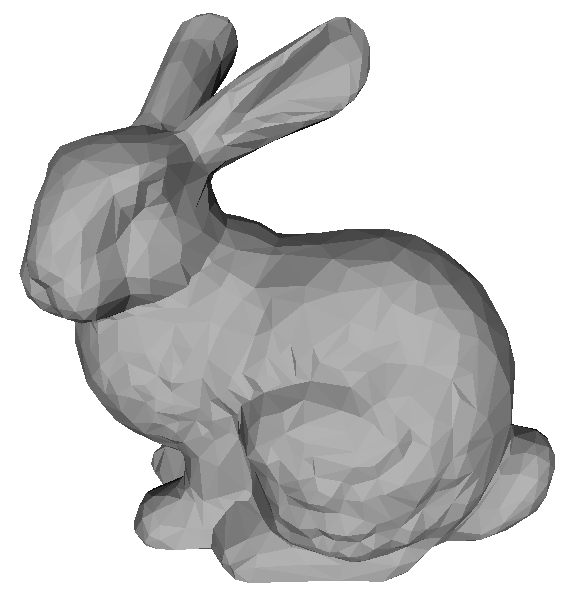
\includegraphics
		[width=0.5\columnwidth]{original_95}\caption{Faces 3642 (5\%)}\label{original_95_ref}\end{subfigure}\\
	\end{tabular}
	\caption{Quality of the simplification of the original mesh.}
  	\label{tab:original_ref}
  	\end{center}
	\end{table}
\end{center}

\begin{center}
  	\begin{table}[H]
  	\begin{center}
  	\begin{tabular}{cc}
	\begin{subfigure}{0.4\textwidth}\centering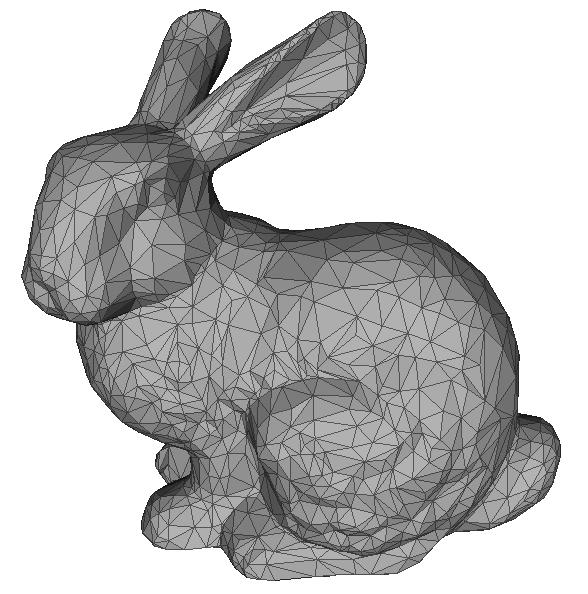
\includegraphics
		[width=0.7\columnwidth]{bunny_100}\caption{Faces 3642}\label{ref_label1}\end{subfigure}&	
	\begin{subfigure}{0.4\textwidth}\centering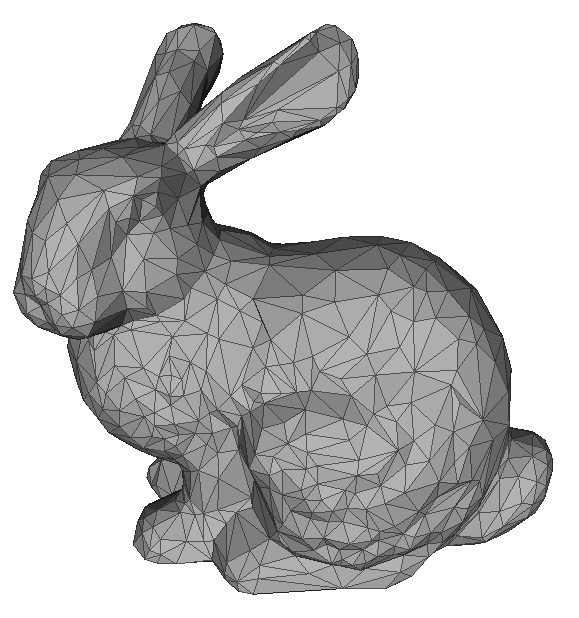
\includegraphics
		[width=0.7\columnwidth]{bunny_80}\caption{Faces 2228}\label{bunny_80_ref}\end{subfigure}\\
	\newline
	\begin{subfigure}{0.4\textwidth}\centering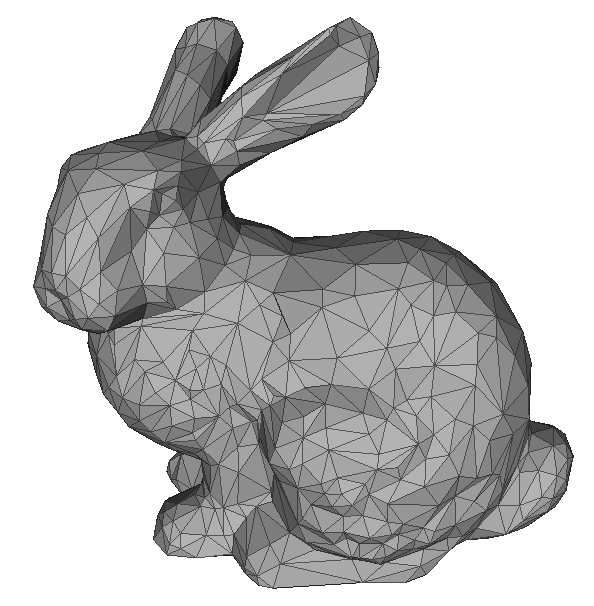
\includegraphics
		[width=0.7\columnwidth]{bunny_70}\caption{Faces 1842}\label{bunny_70_ref}\end{subfigure}&
	\begin{subfigure}{0.4\textwidth}\centering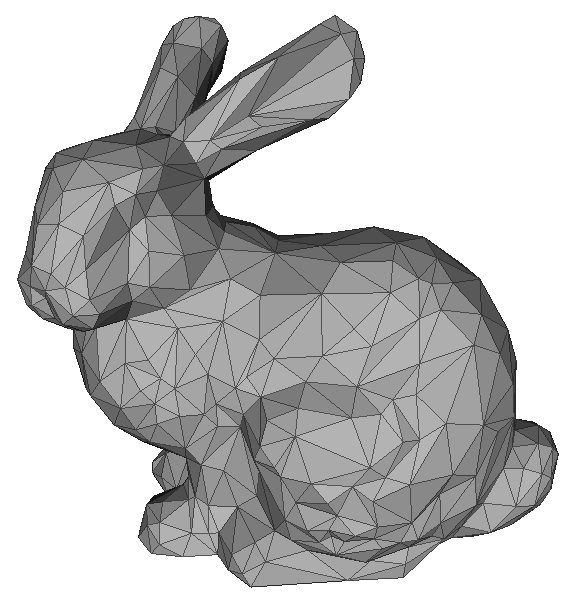
\includegraphics
		[width=0.7\columnwidth]{bunny_60}\caption{Faces 1152}\label{bunny_60_ref}\end{subfigure}\\
	\newline
	\begin{subfigure}{0.4\textwidth}\centering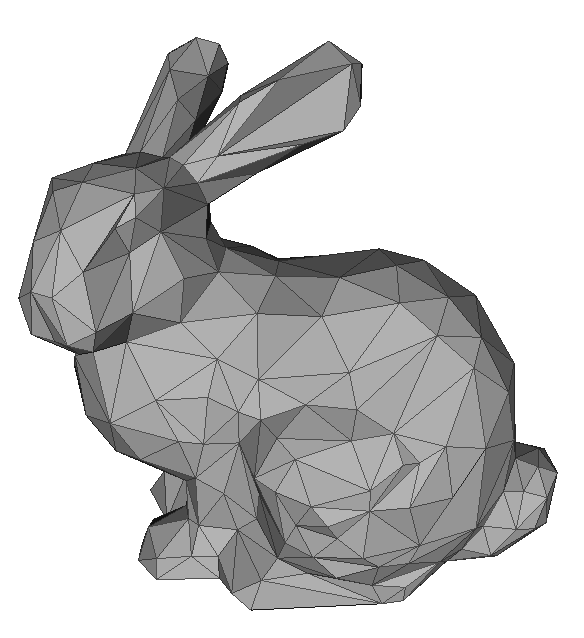
\includegraphics
		[width=0.7\columnwidth]{bunny_50}\caption{Faces 655}\label{bunny_50_ref}\end{subfigure}&
	\begin{subfigure}{0.4\textwidth}\centering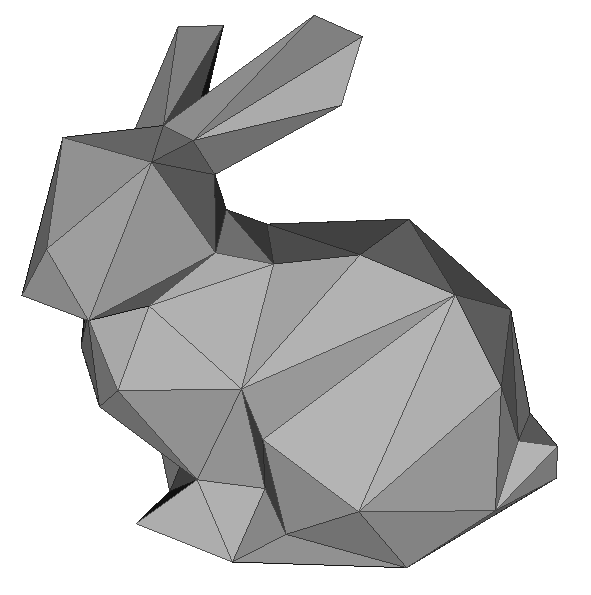
\includegraphics
		[width=0.7\columnwidth]{bunny_40}\caption{Faces 130}\label{bunny_40_ref}\end{subfigure}\\
	\end{tabular}
  	\caption{Several approximations of Stanford Bunny constructed with the geometry quadric error metric.} \label{tab:approx_bunny_ref}
  	\end{center}
	\end{table}
\end{center}

\begin{center}
  	\begin{table}[H]
  	\begin{center}
  	\begin{tabular}{cc}
	\begin{subfigure}{0.4\textwidth}\centering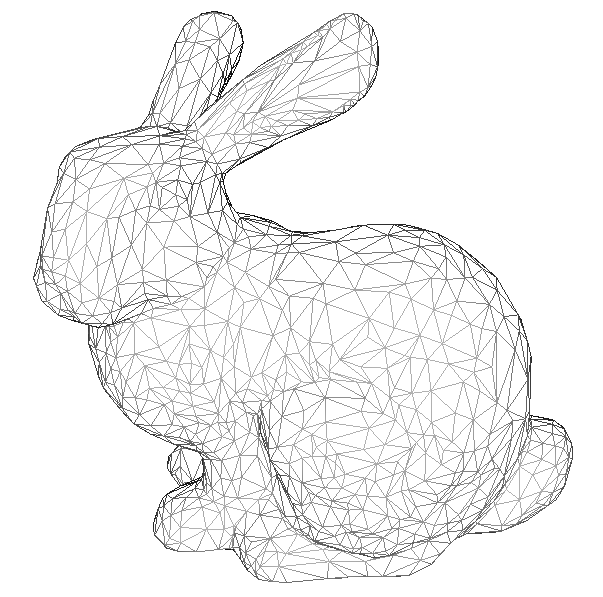
\includegraphics
		[width=0.7\columnwidth]{wireframe_100}\caption{Faces 3642}\label{wireframe_100_ref}\end{subfigure}&	
	\begin{subfigure}{0.4\textwidth}\centering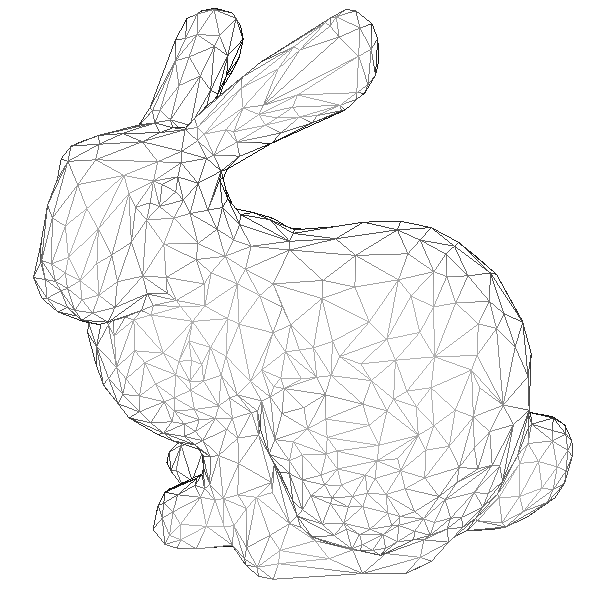
\includegraphics
		[width=0.7\columnwidth]{wireframe_80}\caption{Faces 2228}\label{wireframe_80_ref}\end{subfigure}\\
	\newline
	\begin{subfigure}{0.4\textwidth}\centering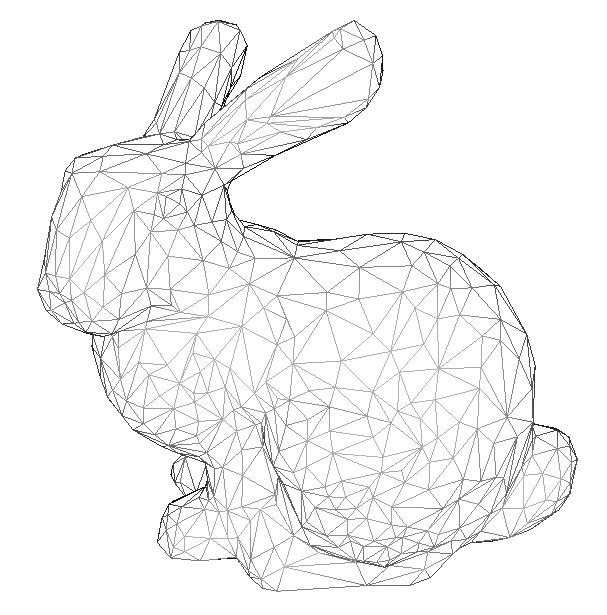
\includegraphics
		[width=0.7\columnwidth]{wireframe_70}\caption{Faces 1842}\label{wireframe_70_ref}\end{subfigure}&
	\begin{subfigure}{0.4\textwidth}\centering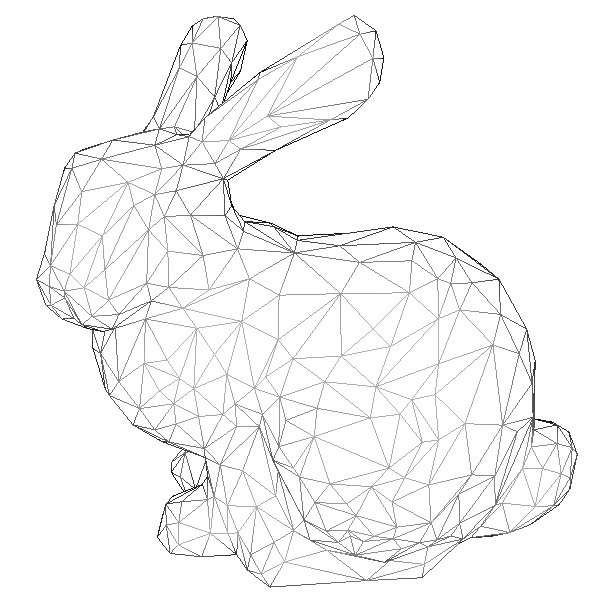
\includegraphics
		[width=0.7\columnwidth]{wireframe_60}\caption{Faces 1152}\label{wireframe_60_ref}\end{subfigure}\\
	\newline
	\begin{subfigure}{0.4\textwidth}\centering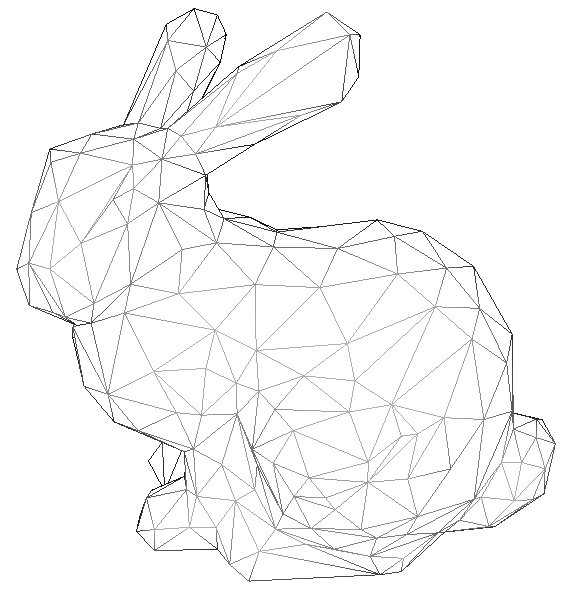
\includegraphics
		[width=0.7\columnwidth]{wireframe_50}\caption{Faces 655}\label{wireframe_50_ref}\end{subfigure}&
	\begin{subfigure}{0.4\textwidth}\centering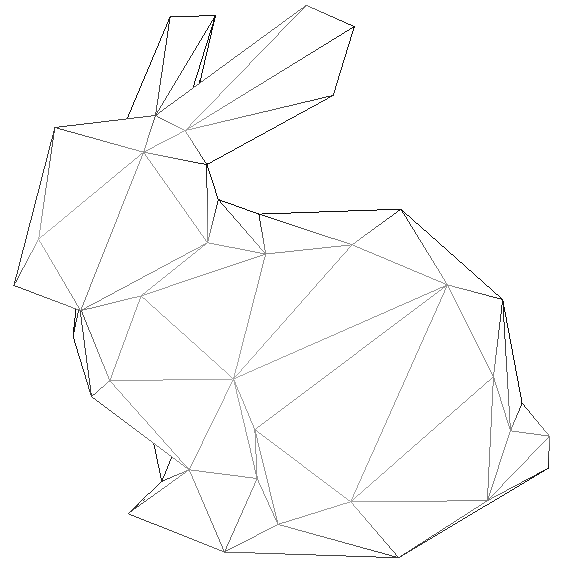
\includegraphics
		[width=0.7\columnwidth]{wireframe_40}\caption{Faces 130}\label{wireframe_40_ref}\end{subfigure}\\
	\end{tabular}
  	\caption{Wireframe versions of models in Table~\ref{tab:approx_bunny_ref}}
  	\label{tab:wireframe_ref}
  	\end{center}
	\end{table}
\end{center}

\newpage
\section{Vertex Placement}

To perform the contraction of an edge $(\mathbf{v_i}, \mathbf{v_j})\rightarrow\bar{\mathbf{v}}$ the calculations of a new position $\mathbf{\bar{v}}$, which is called the target, has to be done. The optimal placement strategy, therefore, is to find a point for which $Q(\mathbf{\bar{v}})$ is minimal. Since, $Q(\mathbf{\bar{v}})$ is quadratic it is guaranteed to find an unique minimizer which is a global minimum.
\begin{align}
Q(\mathbf{v}) &= \mathbf{v}^T\mathbf{A}\mathbf{v} + 2\mathbf{b}^T\mathbf{v} + c\\
\nabla Q(\mathbf{v}) &= 2\mathbf{A}\mathbf{v} + 2 \mathbf{b}
\end{align}
Solving for $\nabla Q(\mathbf{v}) = 0$, the optimal position is defined:
\begin{align}
\mathbf{\bar{v}} = -\mathbf{A}^{-1}\mathbf{b}
\label{v_bar}
\end{align}
and the error:
\begin{align}
Q(\mathbf{\bar{v}}) = \mathbf{b}^T\mathbf{\bar{v}} + c = -\mathbf{b}^T\mathbf{A}^{-1}\mathbf{b} + c
\end{align}

The function used to calculate the optimal position $\mathbf{\bar{v}}$ is the following:
\begin{center}
\begin{lstlisting}[caption={LU decomposition for solving a linear system.},captionpos=b]
virtual bool optimize(Eigen::VectorXd &result) {
	Eigen::FullPivLU<Eigen::MatrixXd> lu = A.fullPivLu();
	if (!lu.isInvertible())
		return false;
	result = -lu.solve(b);
	return true;
};
\end{lstlisting}
\end{center}
Eigen::FullPivLU is LU decomposition of a matrix with complete pivoting, and related features. This decomposition provides the generic approach to solving systems of linear equations, computing the rank, invertibility, inverse, kernel, and determinant \cite{eigenLU19}.

The standard routine is based on 3 basics checks \cite{garland99}:
\begin{enumerate}
\item Try to compute $\mathbf{\bar{v}}$ (\ref{v_bar})
\item If $\mathbf{A}$ is singular, find the optimal position along the line segment $(\mathbf{v_i}, \mathbf{v_j})$, by checking 3 points for the minimum error $[\mathbf{v_i}, \mathbf{v_j}, (\mathbf{v_j} - \mathbf{v_i}) / 2]$.
\item If this is not unique, select the better of $\mathbf{v_i}$ and $ \mathbf{v_j}$.
\end{enumerate}
In practice it is very rare that a matrix determinant is zero. Due to the limits of floating point precision. However, the function $isInvertible()$ determines which pivots should be considerd nonzero, based on a certain threshold defined in the Eigen::FullPivLU implementation. A matrix with determinant close to zero will be considered as not a full-rank matrix \cite{strang88}. Consequently, step 2 or 3 has to be performed to find the optimal point.

The optimal vertex placement will tend to create closely fitting approximations of the original mesh. Therefore, the resulting meshes are shaped in a way that triangles are more equilateral and their areas are more uniform. This method is the best choice for generating fixed approximations of an original \cite{garland99}. 

Summarizing, the general placement strategy for the pair of contraction $(\mathbf{v_i}, \mathbf{v_j})$ is to always move $\mathbf{v_i}$ to $\mathbf{\bar{v}}$ and then $\mathbf{v_j}$ to the position of $\mathbf{v_i}$. It eliminates a problem of storing delta of the new vertex position.

\newpage
\section{Constraints}

Simplification requires several different constrains and checks to not introduce a topology error in the new vertex placement position. The quality of approximation is critical for producing simplified meshes. For instance, the borders of a mesh have to be treated as a special case.

There are a few options the problem of borders can solve. This implementation uses a version with adding the quadric error of a plane perpendicular to a given border edge. The perpendicular plane itself defines a boundary constraint. The other option is to not touch border vertices. However, this option is problematic if a certain level of simplification has to be achieved. The number of border vertices can be even 15\% of the mesh. It means that this 15\% has to be transfered from the complex shapes which we would like to preserve to the simplification pool. Therefore, the quality of the mesh is sacrificed  for the sake of preserving edges.

\begin{figure}[h!]
  \begin{center}
    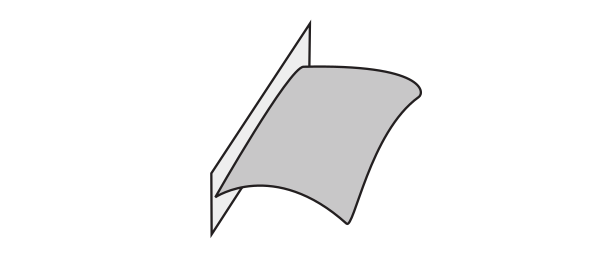
\includegraphics[width=13cm]{border_constraint}
    \caption{An example of the border constrain \cite{garland99}.}
    \label{fig:border_constraint}
  \end{center}
\end{figure}

The perpendicular plane constraint is very convenient in many aspects. For instance, it requires only to calculate the quadric error and add this error to the initial quadric error of each vertex on the boundary. It can be done in the initialization step when the heap is built. After each main iteration, the vertices are flagged if they lay on the border. Once the perpendicular error planes are accumulated in the vertices the algorithm continues the regular routine.

The perpendicular plane constraint can be additionally weighted by an arbitrary constant factor. This implementation do not use the factor multiplication because of the adaptive thresholding, which ignores all edges above the current threshold level. In this version of the algorithm, the edges are consumed as soon as possible to reduce the simplification pool.
\newpage
The other very important problem is vertex folding. A vertex placement can introduce a new position for a vertex which folds the neighborhood and produces degeneracies into the mesh.

\begin{figure}[H]
  \begin{center}
    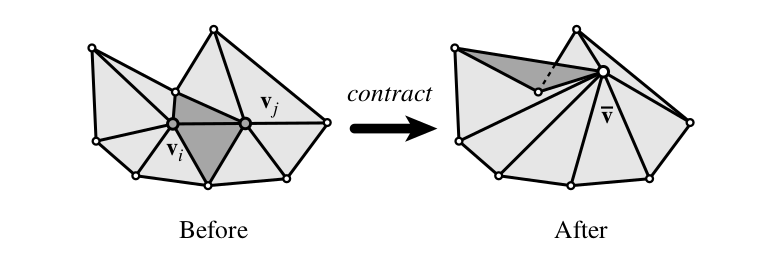
\includegraphics[width=15cm]{fold}
    \caption{An edge contraction which causes the mesh to fold over on itself \cite{garland99}.}
    \label{fig:fold}
  \end{center}
\end{figure}

Before performing a contraction, the algorithm has to check, if the new position is a valid one. For example, Figure \ref{fig:fold} shows the degenerated new position of $\mathbf{\bar{v}}$ which folds one of the faces into the darkened area. In this case, the contraction is stopped for this particular edge. To detect those kind of situations, the normals of faces around $\mathbf{v_i}, \mathbf{v_j}$ are examined. If the face normal changes by some threshold level, the contraction is assumed to introduced flipping and is discarded. 

To determine if a flipping occurred, two checks are preformed. First, checking if the area of newly created face is sufficient. Meaning, investigate the angle between edges. If it is bigger than some threshold, edges are almost co-linear. If a triangle is defined as $T = (\mathbf{p}, \mathbf{q}, \mathbf{r})$ then:

\begin{figure}[H]
  \begin{center}
    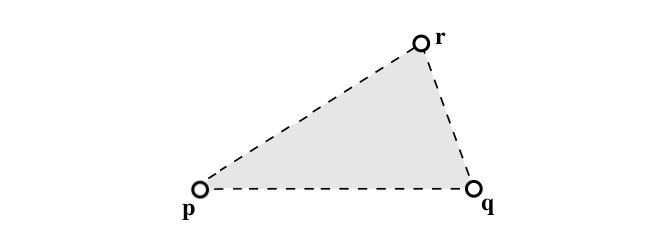
\includegraphics[width=11cm]{triangle}
    \caption{Triangle $T = (\mathbf{p}, \mathbf{q}, \mathbf{r})$.}
    \label{fig:gram}
  \end{center}
\end{figure}

\begin{align}
\mathbf{u} &= \frac{\mathbf{r} - \mathbf{\bar{v}}}{\norm{\mathbf{r} - \mathbf{\bar{v}}}}\\
\mathbf{v} &= \frac{\mathbf{q} - \mathbf{\bar{v}}}{\norm{\mathbf{q} - \mathbf{\bar{v}}}}\\
t &= |\mathbf{u} \cdot \mathbf{v}|
\end{align}
where $\mathbf{u}$ and $\mathbf{v}$ are unit vectors and $\mathbf{\bar{v}}$ is the new optimal position. Variable $t$ caries the notion of angle between two vectors, if $t$ is bigger than $0.999$ the flipping was introduced and two new edges are very close to be co-linear.

\begin{figure}[H]
  \begin{center}
    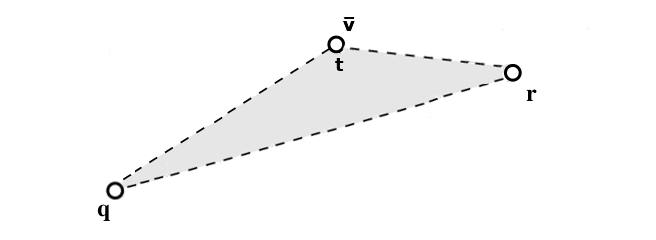
\includegraphics[width=11cm]{triangle_angle}
    \caption{A new triangle $T = (\mathbf{q}, \mathbf{r}, \mathbf{\bar{v}})$  where $t$ is the angle used to check the co-linearity constraint.}
    \label{fig:gram}
  \end{center}
\end{figure}

\newpage
The second check investigates normals Figure \ref{fig:border_constraint}. Using previously defined vectors $\mathbf{u}$ and $\mathbf{v}$ and triangle $T$ with its normal as $\mathbf{n}_T$ the definition is as follows:
\begin{align}
\mathbf{n} &= \frac{ \mathbf{u} \times \mathbf{v}}{\norm{\mathbf{u} \times \mathbf{v}}}\\
c &= \mathbf{n} \cdot \mathbf{n}_T
\end{align}

If $c$ is smaller than $0.2$ the contraction is rejected. Basically, it means that the new face is going to flip and is close to be perpendicular to the neighboring face. In many cases it introduces inconsistencies. In this situation the removal is also rejected.

To correctly investigate flipping, the whole silhouette of neighbors of a given new vertex position has to be checked. The test check has to pass for all of them to accept a decimation.

\newpage
\section{Summary of Garland's Algorithm}

Below, the complete algorithm in 5 steps is presented. The next chapter elaborates how this concept is incorporated in multi-threaded approach.

Algorithm \cite{garland99}:

\begin{enumerate}
\item Select a set of candidate vertex pairs $(\mathbf{v_i}, \mathbf{v_j})$.
\item Allocate a quadric $Q_i$ for each vertex $\mathbf{v_i}$.
\item For each face compute a quadric $Q_i$. Add this fundamental quadric to the vertex quadrics $Q_i, Q_k, Q_l$ and optionally weight it appropriately.
\item For each candidate pair $(\mathbf{v_i}, \mathbf{v_j})$:
\begin{enumerate}
\item Compute $Q = Q_i + Q_j$.
\item Select a target position $\mathbf{\bar{v}}$.
\item Apply consistency checks and penalties.
\item Place pair in heap keys on cost $Q(\mathbf{\bar{v}})$
\end{enumerate}
\item Repeat until the desired approximation is reached:
\begin{enumerate}
\item Remove the pair $(\mathbf{v_i}, \mathbf{v_j})$ of least cost from the heap.
\item Preform contraction $(\mathbf{v_i}, \mathbf{v_j})\rightarrow\bar{\mathbf{v}}$
\item Set $Q_i = Q_i + Q_j$.
\item For each remaining pair $(\mathbf{v_i}, \mathbf{v_j})$, compute target position and cost as in step 4; update heap.
\end{enumerate}
\end{enumerate}

The algorithm above is the main core of the implementation. Every thread will perform the simplification using quadric error metrics, based on Garland's work. In the next chapter, a brief introduction to the extended version of the algorithm which includes color and normals is given.

\chapter{Extended Simplification Algorithm}

The previous implementation includes only geometric error. In this chapter more attributes to improve simplification are incorporated. Using additionally color and normals, the decimation of planar surfaces can be easier achieved and gives better results. However, in the noisy environment of color (which is usually the case in scans), gradient guided simplification may affect the results.

\section{Design}
In this section, the main assumption is that each vertex is additionally associated with color $\mathbf{c} = [r \ g \ b]^T$ and normal $\mathbf{n} = [nx \ ny \ nz]^T$. For the sake of simplicity, lets consider an example with geometry and color only. Assume that each vertex is attributed with $\mathbf{v} = [x \ y \ z \ r \ g \ b]^T$. Figure~\ref{fig:hexagon} shows an example of a mesh like that. A triangle is defined as $T = (\mathbf{p}, \mathbf{q}, \mathbf{r})$ with edges $\mathbf{h} = \mathbf{q} - \mathbf{p}$ and $\mathbf{k} = \mathbf{r} - \mathbf{p}$. Since the input vector for the optimization are more then 3 dimensional, a different method to calucalte orthogonal vectors to the plane defined by the face is used. Simply calculating a cross product of two vectors will not work. Gram-Schmidt vectors orthogonalization method solves this problem \cite{strang88}.

\begin{figure}[H]
  \begin{center}
    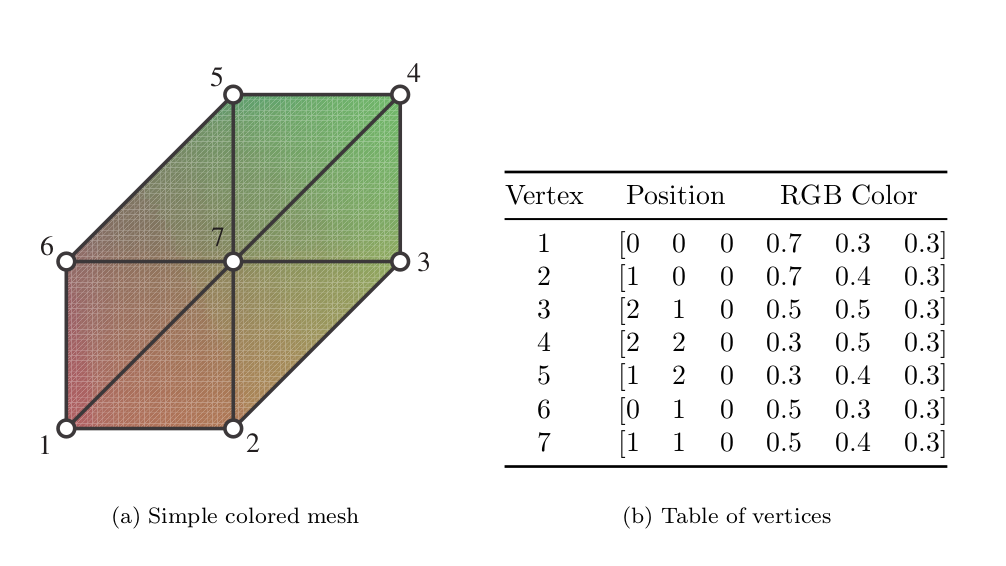
\includegraphics[width=15cm]{hexagon}
    \caption{A triangulated hexagon with color values at each vertex \cite{garland99}.}
    \label{fig:hexagon}
  \end{center}
\end{figure}

Therefore, two orthogonal to each other vectors $\mathbf{e_1}, \mathbf{e_2}$ are defined as:

\begin{align}
\mathbf{e_1} &= \mathbf{h} / \norm{\mathbf{h}} \\
\mathbf{e_2} &= \frac{\mathbf{k} - (\mathbf{e_1} \cdot \mathbf{k})\mathbf{e_1}}{\norm{\mathbf{k} - (\mathbf{e_1} \cdot \mathbf{k})\mathbf{e_1}}}
\end{align}

$\mathbf{e_1}, \mathbf{e_2}$ are unit-length vectors which form a local coordinate system with $\mathbf{p}$ as the origin. Those vectors describe a plane like object in $\mathbb{R}^6$.

\begin{figure}[H]
  \begin{center}
    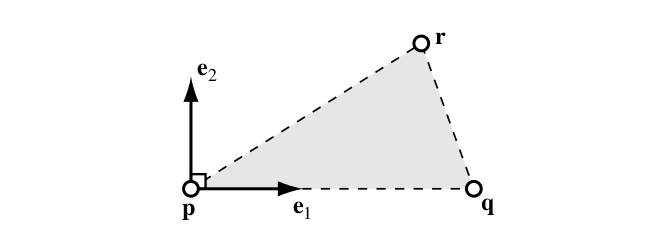
\includegraphics[width=12cm]{gram}
    \caption{Orthonomal vectors \cite{garland99}.}
    \label{fig:gram}
  \end{center}
\end{figure}

Now, the distance from an arbitrary point $\mathbf{v}\in\mathbb{R}^n$ to the plane created by the face $T$ will be presented. The squared distance of the vector $\mathbf{u} = \mathbf{p} - \mathbf{v}$ is defined as \cite{garland99}:

\begin{align}
\norm{\mathbf{u}}^2 = \mathbf{u}^T\mathbf{u} = (\mathbf{u}^T\mathbf{e_1})^2 + ... +  (\mathbf{u}^T\mathbf{e_n})^2
\end{align}

Rearranging the equation gives:

\begin{align}
(\mathbf{u}^T\mathbf{e_3})^2 + ... +  (\mathbf{u}^T\mathbf{e_n})^2 = \norm{\mathbf{u}}^2 - (\mathbf{u}^T\mathbf{e_1})^2 - (\mathbf{u}^T\mathbf{e_2})^2
\end{align}

The left hand side is the squared distance of $\mathbf{u}$ along all the axes perpendicular to the plane of $T$. This is the distance between this vector $\mathbf{v}$ and the plane $T$.

\begin{align}
D^2 = \mathbf{u}^T\mathbf{u} - (\mathbf{u}^T\mathbf{e_1})(\mathbf{u}^T\mathbf{e_1}) - (\mathbf{u}^T\mathbf{e_2})(\mathbf{u}^T\mathbf{e_2})
\end{align}

The quadric metric is defined as $Q(\mathbf{v}) = \mathbf{v}^T\mathbf{A}\mathbf{v} + 2\mathbf{b}^T\mathbf{v} + c$ where:

\begin{align}
\mathbf{A} &= \mathbf{I} - \mathbf{e_1}\mathbf{e_1}^T - \mathbf{e_2}\mathbf{e_2}^T\\
\mathbf{b} &= (\mathbf{p} \cdot \mathbf{e_1})\mathbf{e_1} + (\mathbf{p} \cdot \mathbf{e_2})\mathbf{e_2} - \mathbf{p}\\ 
\mathbf{c} &= \mathbf{p} \cdot \mathbf{p} - (\mathbf{p} \cdot \mathbf{e_1})^2 - (\mathbf{p} \cdot \mathbf{e_2})^2 
\end{align}

For more details please refer to Michael Garland's Quadric-Based Polygonal Surface Simplification.

The matrix $\mathbf{A}$ from \ref{fig:hexagon} is then:

\begin{align}
\left[
\begin{array}{rrrrrr}
0.06 & 0 & 0 & 0 & -0.59 & 0\\
0 & 0.23 & 0 & 1.15 & 0 & 0\\
0 & 0 & 6.00 & 0 & 0 & 0\\
0 & 1.15 & 0 & 5.77 & 0 & 0\\
-0.59 & 0 & 0 & 0 & 5.94 & 0\\
0 & 0 & 0 & 0 & 0 & 6.00
\end{array}\right]
\end{align}

Building the quadric and finding the optimal position is exactly the same like in the geometry case. To use a different metric, a proper orthonormal vectors in $\mathbf{R}^n$ have to be provided.

\begin{figure}[H]
  \begin{center}
    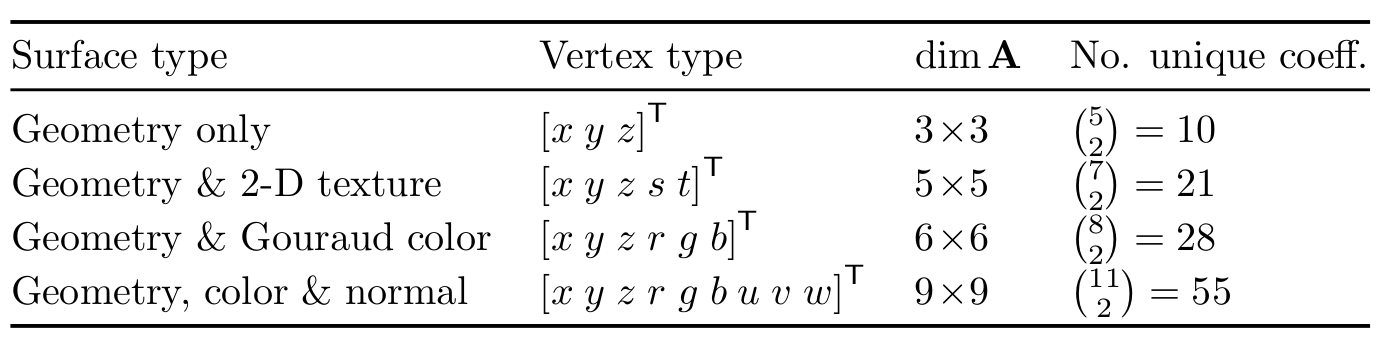
\includegraphics[width=15cm]{params_table}
    \caption{Summary of common extended quadric types \cite{garland99}.}
    \label{fig:params_table}
  \end{center}
\end{figure}

\section{Results}

As it can be seen in the Table \ref{tab:desk}, complex shapes like plants or a small fan in front of the monitor preserve their initial complexity. However, flat surfaces like the desk or the monitor are significantly simplified. Therefore, the amount of removable faces, to achieve a particular simplification level, was transfered from the complex shapes pool to the flat surface pool. Complex shapes will be simplified only in the case when planar surfaces are as simply as possible and removal is not longer available.

Table \ref{tab:color_simplification} shows the results of using color and geometry metric error. It can be easily noticed that the simplification follows the color pattern. In some cases it is a desired features, however, since the color distribution on planar surfaces is typically non-uniform, the resulting color gradients might have undesired impact on the final simplification result.

If the color gradient was constant in most of the places, the whole simplification would hugely benefit from it. However, not only a camera introduces an error, in the case of $3D$ datasets captured by mobile lasers scanners like the NavVis $M6$, error sources as calibration and SLAM need to be considered when choosing the right attributes for the simplification. Therefore, either normals, color, geometry are incorporated all together or used separately.

\begin{center}
  	\begin{table}[H]
  	\begin{center}
  	\begin{tabular}{cc}
	\begin{subfigure}{0.8\textwidth}\centering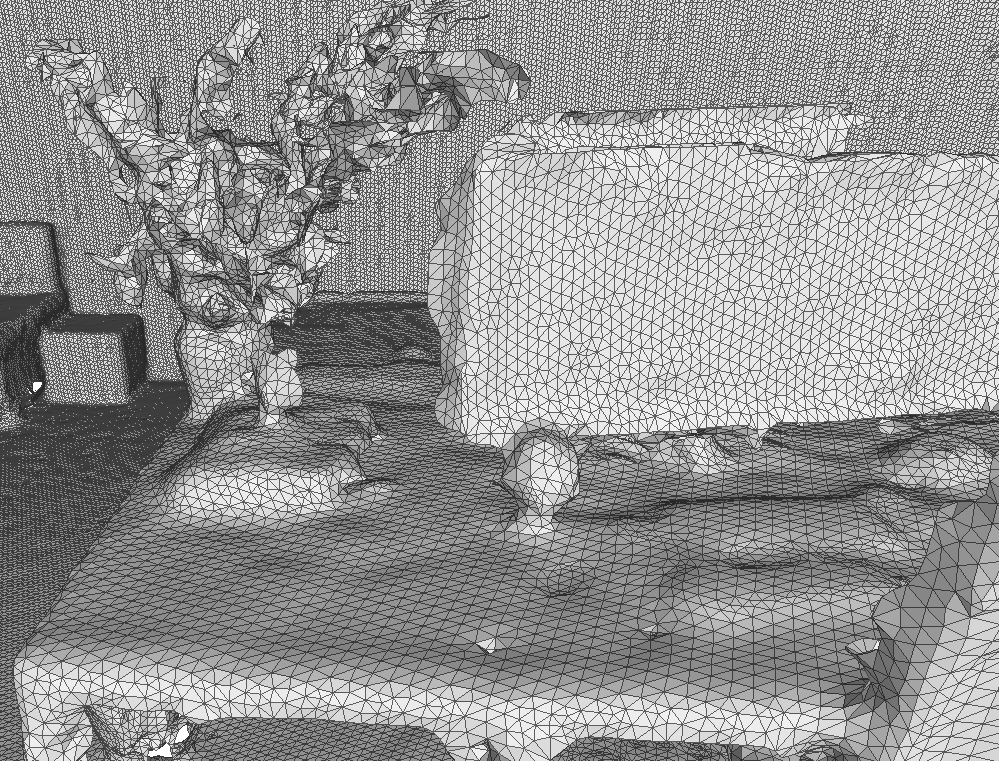
\includegraphics
		[width=1\columnwidth]{desk_2}\caption{Original}\label{original_100_ref}\end{subfigure}\\
	\begin{subfigure}{0.8\textwidth}\centering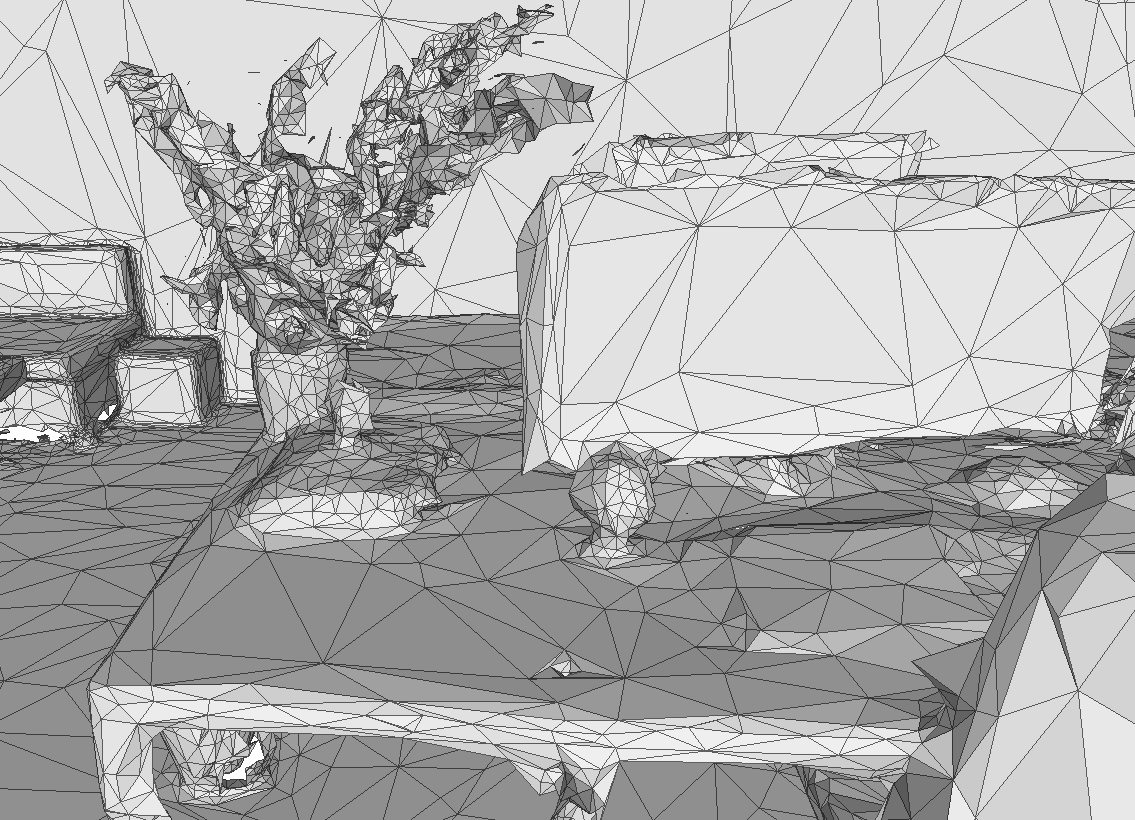
\includegraphics
		[width=1\columnwidth]{desk}\caption{Color, geometry and normal simplification}\label{original_70_ref}\end{subfigure}\\
	\end{tabular}
	\caption{Comparison of simplification with all attributes [geometry, color, normal] with 87\% of reduction to the original mesh.}
  	\label{tab:desk}
  	\end{center}
	\end{table}
\end{center}

\newpage
\begin{center}
  	\begin{table}[H]
  	\begin{center}
  	\begin{tabular}{cc}
	\begin{subfigure}{0.5\textwidth}\centering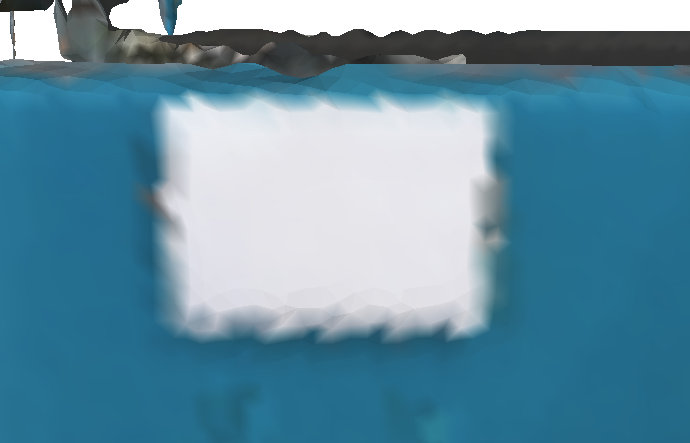
\includegraphics
		[width=7cm,height=5cm]{color_1}\caption{Original.}\label{color1}\end{subfigure}&	
	\begin{subfigure}{0.5\textwidth}\centering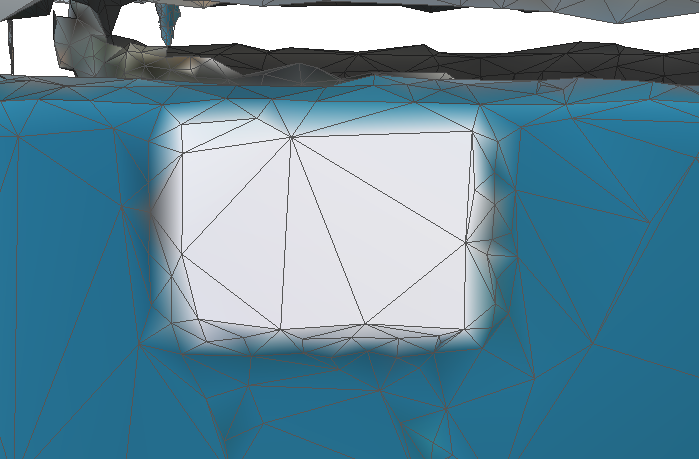
\includegraphics
		[width=7cm,height=5cm]{color_2}\caption{Color and geometry simplification.}\label{color2}\end{subfigure}\\
		\newline
			\begin{subfigure}{0.5\textwidth}\centering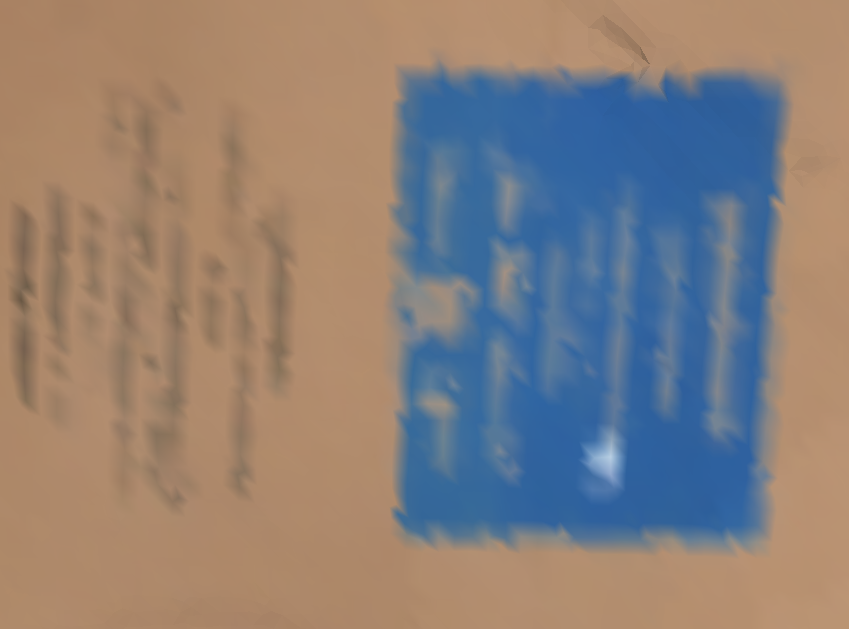
\includegraphics
		[width=7cm,height=5cm]{color_4}\caption{Original.}\label{color1}\end{subfigure}&	
	\begin{subfigure}{0.5\textwidth}\centering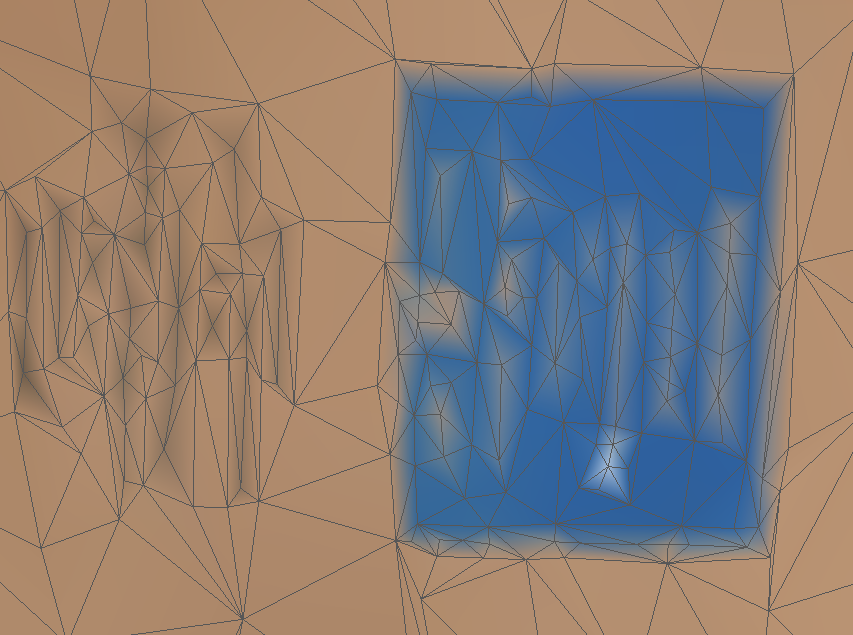
\includegraphics
		[width=7cm,height=5cm]{color_3}\caption{Color and geometry simplification.}\label{color2}\end{subfigure}\\
				\newline
			\begin{subfigure}{0.5\textwidth}\centering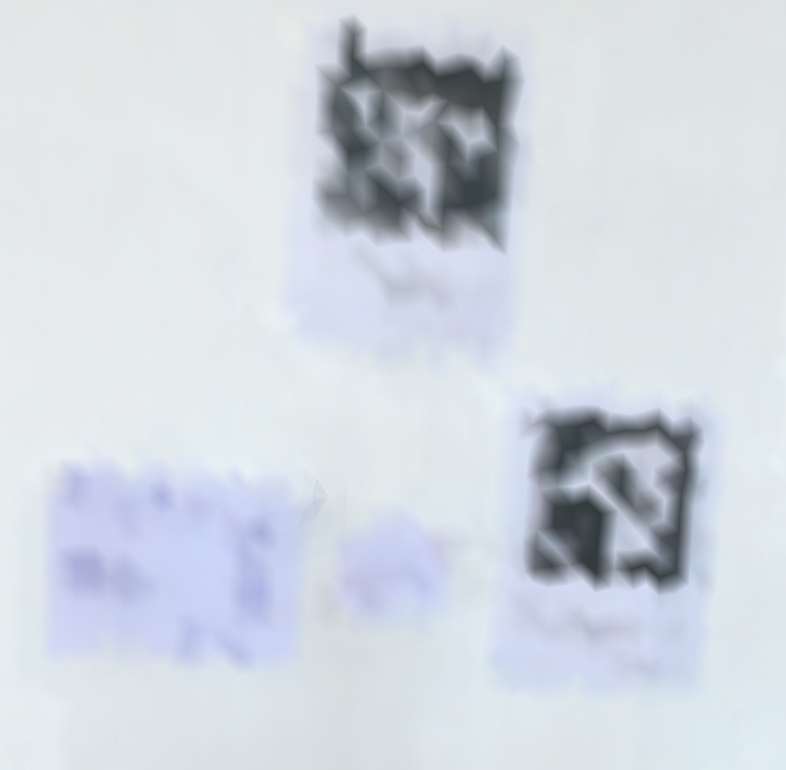
\includegraphics
		[width=7cm,height=5cm]{color_5}\caption{Original.}\label{color1}\end{subfigure}&	
	\begin{subfigure}{0.5\textwidth}\centering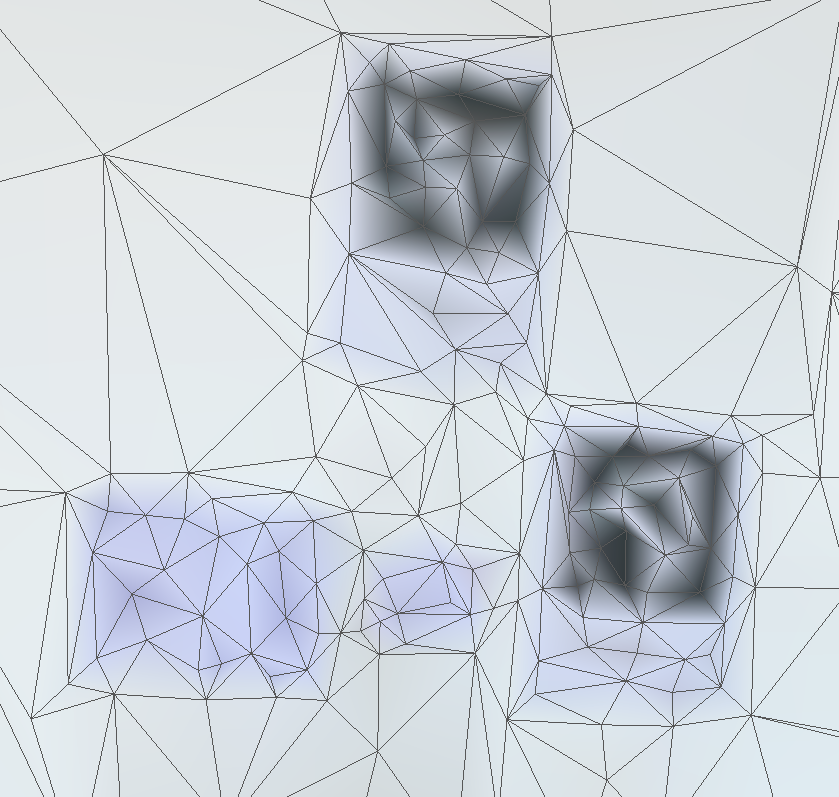
\includegraphics
		[width=7cm,height=5cm]{color_6}\caption{Color and geometry simplification.}\label{color2}\end{subfigure}\\
	\begin{subfigure}{0.5\textwidth}\centering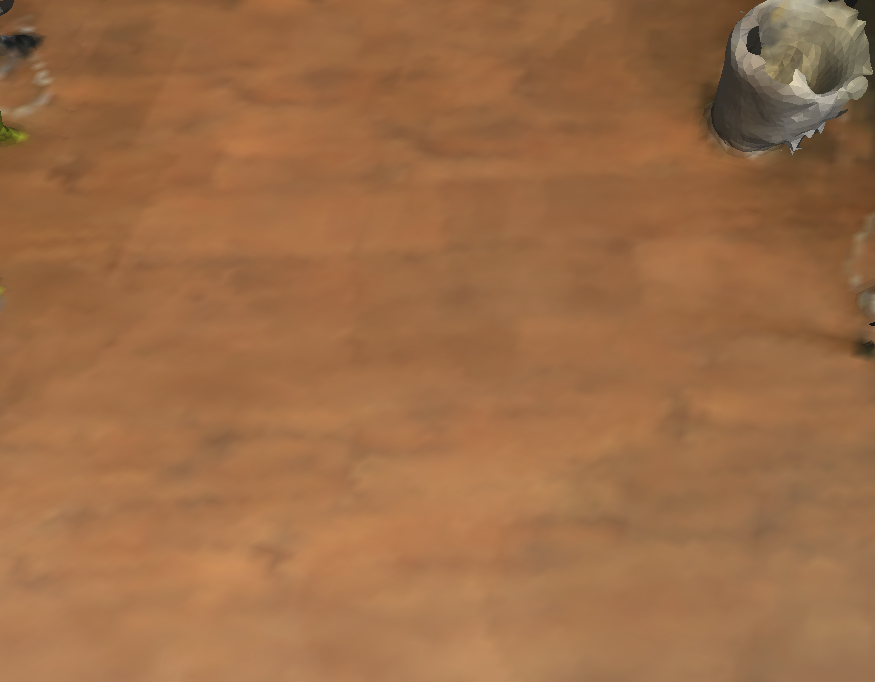
\includegraphics
		[width=7cm,height=5cm]{nosiy_floor_2}\caption{Original floor with color noise.}\label{color1}\end{subfigure}&	
	\begin{subfigure}{0.5\textwidth}\centering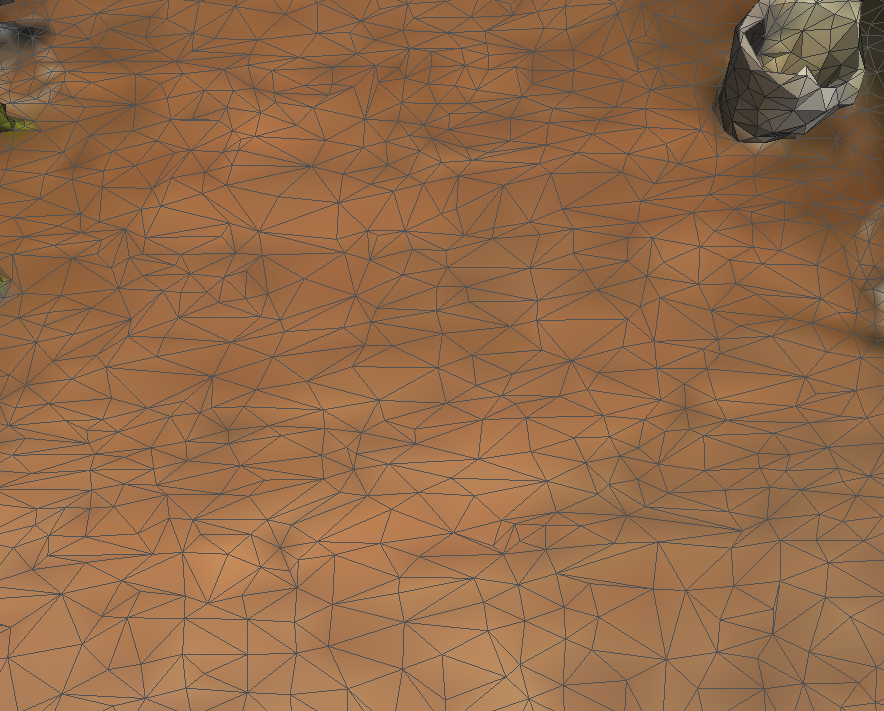
\includegraphics
		[width=7cm,height=5cm]{nosiy_floor}\caption{Gradient guided simplification error.}\label{color2}\end{subfigure}
		\end{tabular}
  	\caption{Comparison of gradient guided simplification [geometry, color].} \label{tab:color_simplification}
  	\end{center}
	\end{table}
\end{center}


\chapter{Parallel Simplification Algorithm}

This chapter introduces the approach to design a parallel version of Garland's simplification algorithm. First, the Producer-Consumer design pattern with libraries and the implementation ideas making it thread-safe are described. Next, the analysis of the speedup and potential problems which can arose during an execution are shown. Finally, summary of the approach and comparison to different algorithms is given.

\section{Producer Consumer Pattern}

The producer-consumer pattern is an optimal way to distribute workload of processing data to worker threads which process the data. In other words, it divides the problem into two major components, connected usually by a queue. This is a classic example of a multi-process synchronization problem. The process separation gives clear view at the problem and tasks. A producer is placing items in a queue, and a consumer removes each task from the queue and processes the data. This decoupling means that two components are completely independent \cite{grand02}. In the case when the queue is full, locking procedure is used to wait for consumers to process tasks.

\begin{figure}[H]
  \begin{center}
    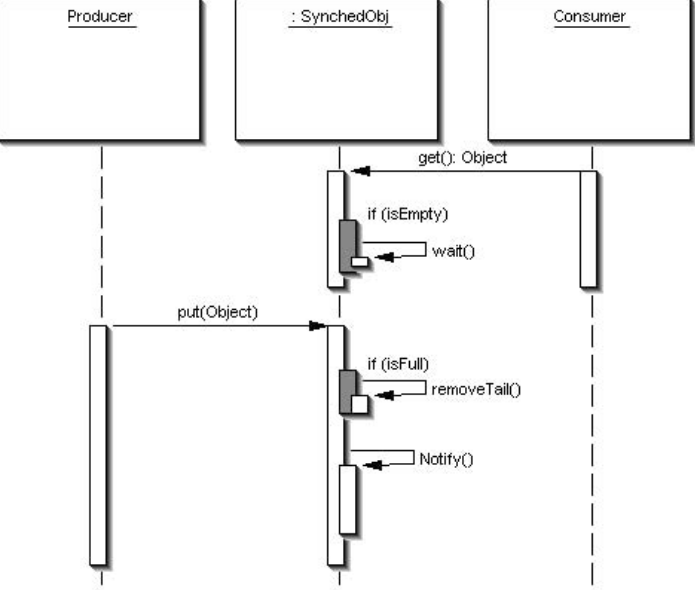
\includegraphics[width=12cm]{producer_consumer}
    \caption{UML sequence diagram for the procuder-consumer pattern implementation \cite{ropero17}.}
    \label{fig:uml}
  \end{center}
\end{figure}

Figure \ref{fig:uml} shows how such a process could look like. Three main components are shown; producer, synchronization object (the queue) and consumer. In the case when the buffer is either full or empty, waiting spin\footnote{A procedure to constantly check if the queue has new tasks to process. This is a common technique used in parallel programming.} is used to hold execution till the moment when more tasks are available for a consumer.

In this implementation a generalized version of the pattern is used, which assumes multiple producers and consumers operating on a single fixed buffer. The main idea is to create separate tasks, which later are consumed by active threads from the thread-pool\footnote{A thread pool is a group of pre-instantiated, idle threads which stand ready to be given work, in this case simplification tasks from the queue.}. To create those tasks, clustering of the mesh is introduced.

\newpage
\section{Producer Design}

To cluster a mesh into sub-boxes, a simple method of dividing the global bounding box is used. When the mesh is read, the global bounding box is calculated, which later is divided into predefined number of clusters.

\begin{figure}[H]
  \begin{center}
    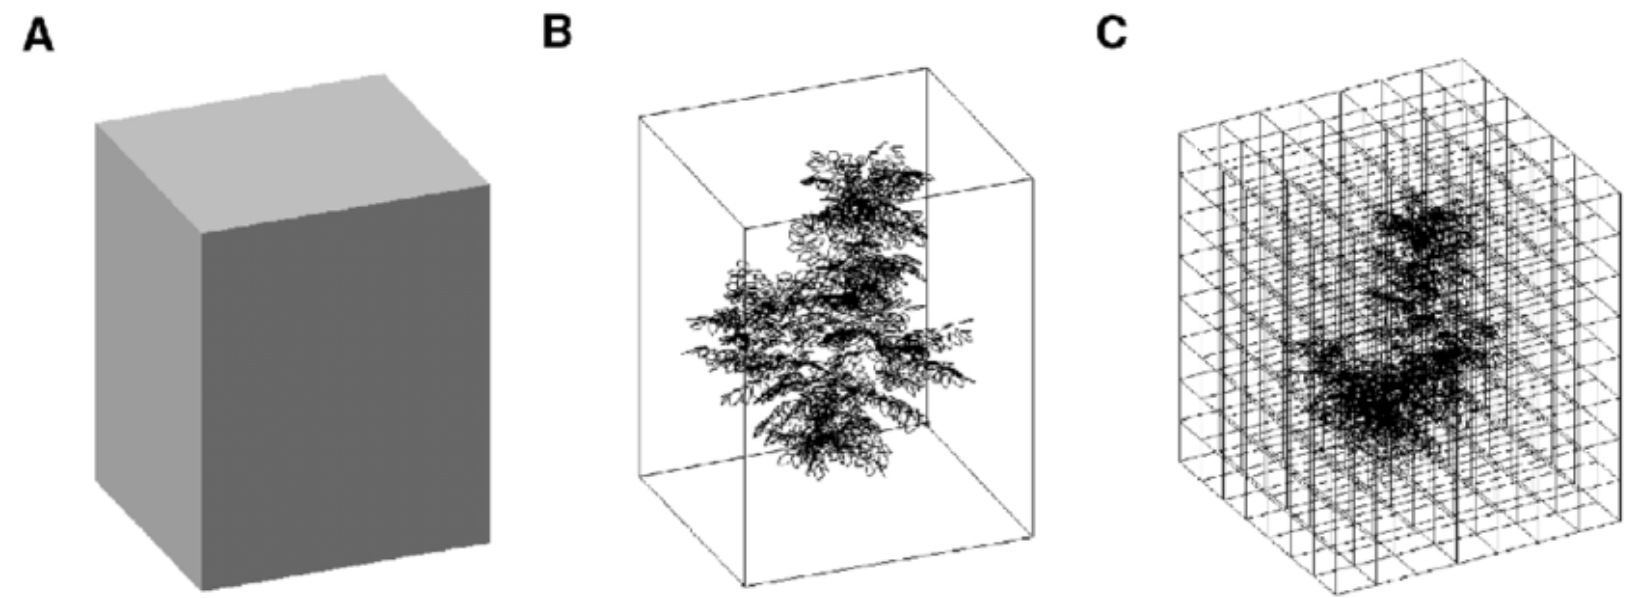
\includegraphics[width=13cm]{clustering}
    \caption{Example of clustring a mesh into 7x7x7 clusters.}
    \label{fig:clustering}
  \end{center}
\end{figure}

Figure \ref{fig:clustering} shows an example with arbitrary $7x7x7=343$ clusters, where each dimension of the main bounding box $[B]$ was divided into 7 equal parts $[C]$. When clustered boxes are calculated, the membership check to which cluster a face belongs is performed. In the case when a face intersects multiple clusters a voting procedure is done, which is defined as follows; if two vertices of a face belong to the same cluster this cluster is selected as a holder of the face. If each vertex belongs to a different cluster then one box is randomly selected. The pseudocode of the producer is the following:
\newline
\begin{center}
\begin{lstlisting}[caption={C style psuedocode of a producer.},captionpos=b]
void function produce {
    clusters = getClusters(size, mesh);
    for (cluster : clusters){
        set faceCluster to empty
        for (face : cluster.elements){
            if vote(face) is true
                add face to faceCluster
        }
        add faceCluster to queue
    }
};
\end{lstlisting}
\end{center}

In the line 6 the $vote()$ function is used to assign the correct cluster $id$ and membership of a face. The line 9 inserts the $faceCluster$ to the queue for further processing.

\newpage
\section{Consumer Design}

The consumer process is designed in a way to utilize funcionality of $\inlinecode{Java}{boost::thread_group}$ and $\inlinecode{Java}{boost::asio::io_service}$. The thread group is a class which helps with thread management and provides a container for easy grouping of threads to simplify several common thread creation and management idioms \cite{boost03}. A user has to specify how many threads will be created and added to the thread-pool. Those threads operate directly on the queue, removing tasks and processing data. In this case they are preforming simplification of a mesh on each cluster independently.
\newline
\begin{center}
\begin{lstlisting}[caption={C style psuedocode of a task for a consumer.},captionpos=b]
void function task {
    garland = QSlim();
    garland->setClustersAABBs();
    garland->initialize<QuadricError>();
    garland->simplify<QuadricError>();
};
\end{lstlisting}
\end{center}

Each task gets a single cluster to process. The $QuadricError$ is a type of a quadric error metric which specifies attributes for the calculations like; geometry, color, normals. The class $QSlim$ is responsible for all simplification operations and was elaborated in the previous sections.

All decimating operations executed by threads are independent, except those on the borders. If one vertex of a face belongs to a different cluster and this cluster is processed by a different thread, a clever locking strategy has to be used. The main idea is to lock\footnote{Locking is a synchronization mechanism for enforcing limits on access to a resource in an environment where there are many threads of execution.} the whole neighborhood of an edge. To avoid deadlocks, a Boost specialized version of $\inlinecode{Java}{boost::recursive_mutex}$ is used. It allows to be locked multiple times by the same thread. In the border situation, the best solution for obtaining a lock is to use the method $\inlinecode{Java}{bool try_lock()}$ which returns immediately false if the mutex is already locked by a different thread. It means that the given neighborhood is already processing by a different thread and the simplification process for the current thread is terminated because the edge is deleted by a different process.

$\inlinecode{Java}{boost::asio::io_service}$ is responsible for the whole producer consumer work-flow and is the centerpiece in this implementation. The service nicely utilizes functionality of a thread-pool. The method $post()$ creates tasks and pushes them to the queue where later they are processed by threads from the thread-pool.

\newpage
\section{Design}

The algorithm is based on Garland's simplification quadric error metric algorithm. The main difference is clustering and parallel consuming parts of a mesh with adaptive thresholding for each iteration. This approach guarantees global update and accumulation of quadrics for each iteration in such a way that planar surfaces are always decimated first. The main goal of this work, is to transfer from a global pool of vertices for a mesh to two separate pools, one for complex shapes and one for planar surfaces. Vertex pools are just conceptual terms which mean the number of vertices which we want to remove to achieve our convergence criteria. However, to retain complex shapes intact, vertices from planar surfaces have to be removed as much as possible to maintain a given trade-off in pools. Therefore, the outer loop of the algorithm, which increases the threshold level, is crucial. The reconstruction always creates a mesh with evenly distributed triangles. This assumption drives the design of the algorithm. Complex shapes have high quadric error. An appropriately manipulated threshold can achieve the desired transfer goal.

To improve time of the simplification convergence, aggressiveness can be increased. The only problem is the final quality of the approximation. The iterative nature of using Garland's algorithm and adaptive thresholding, which targets only planar surface, does not always hold in this case. However, it allows to save around 50\% time of processing by slightly increasing aggressiveness.

\newpage
\section{Results}

This section elaborates results of multi-threaded experiments of the algorithm. Additionally, the time investigation of each execution in multiple scenarios is shown. The tests were performed on a machine with 32 GB of RAM and Intel i7-6700 CPU 3.40GHz with 4 physical cores on a mesh with 982624 faces and 517715 vertices. Six different setups were ran with the objective to achieve a reduction level of 85\% of the original mesh:

\begin{table}[h!]
\centering
\begin{tabular}{ |c|c|c| } 
 \hline
 Number of clusters & Number of threads in the pool & Total time processing\\
 \hline
 1 & 1 & 127.62s\\
 8 & 2 & 77.98s\\
 8 & 4 & 56.77s\\
 8 & 8 & 62.01s\\
 27 & 8 & 48.88s\\
 27 & 27 & 48.02s\\
 \hline
\end{tabular}
\caption{4 different test setups.}
\end{table}

\begin{figure}[h!]
  \begin{center}
    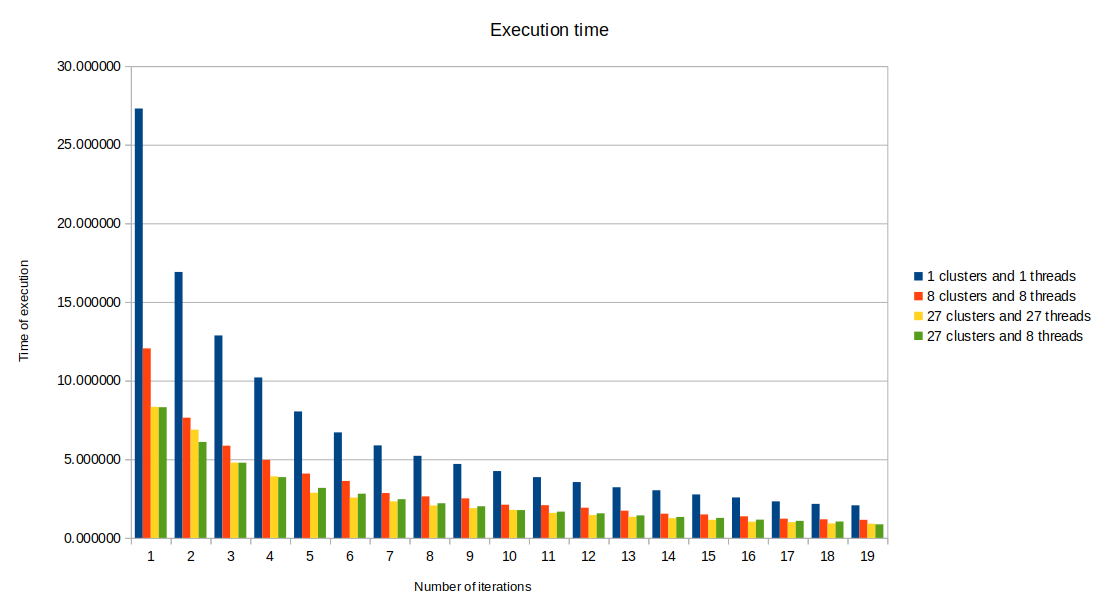
\includegraphics[width=18cm]{chart}
    \caption{Time of execution in seconds with different number of threads and clusters.}
    \label{fig:execution_time}
  \end{center}
\end{figure}

The Figure \ref{fig:execution_time} shows how much time does it take to simplify a mesh in one iteration. In total, there were 19 iterations to achieve the 85\% of simplification. One iteration in this case, is the full pass of the simplification algorithm. It means; to wait for all active threads to finish processing the sub-meshes. Naturally, the time is getting smaller with each iteration because of less vertices to process. As it is expected, the single threaded version performs very poorly. Using more than 1 thread can achieve better results with the best speedup of around 3.5.

\begin{figure}[H]
  \begin{center}
    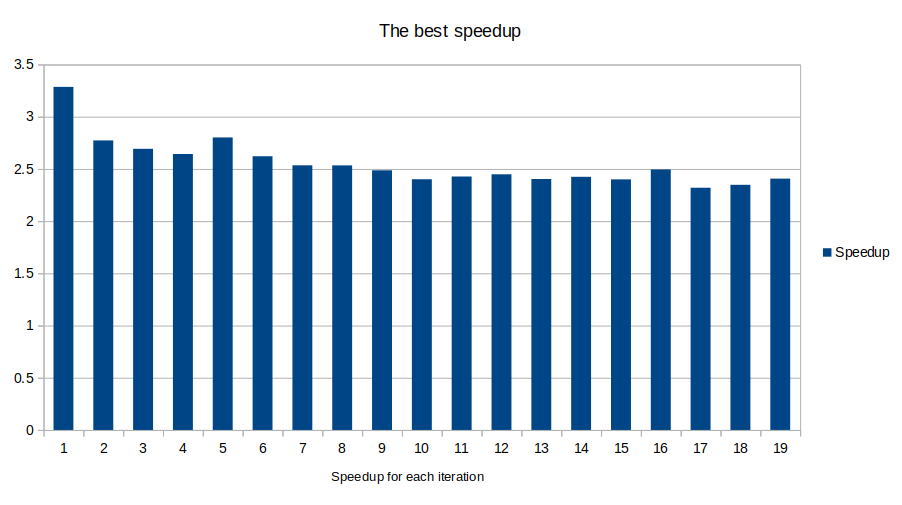
\includegraphics[width=16cm]{chart2}
    \caption{The best speedup for each iteration}
    \label{fig:speedup}
  \end{center}
\end{figure}

The Figure \ref{fig:speedup} desciribes the best speedup for each iteration. The value oscillates around 2.5 and 3 which is a decent result for this complex algorithm. Moreover, in the Figure \ref{fig:execution_time} the Amdahl's law is visible in practice. Incerasing number of threads does not improve speedup \cite{amdahl67}.

To avoid synchronization overhead deep copying of a sub-meshes was tried. Those deeply copied sub-meshes were passed to the processing threads. The problem with this solution is merging sub-meshes into the master mesh after simplification. To preserve local geometry on the edges, the process of decimation need not to change or remove them, which gives a rise to the problem with convergence. Moreover, merging meshes takes time and the algorithm does not gain much performance speedup using this strategy.

Summarizing, the parallel execution of clusters gives a desired speedup. The algorithm is able to process big meshes up to a few million of faces in reasonable time, which is necessary for streaming purposes and production usage.

\newpage
\section{Taubin Smoothing}

During the research and later implementation of the algorithm, faster convergance to selected level of reduction was noticed when the input mesh was smoothed in a pre-processing step. For purposes of this work, Taubin Smoothing algorithm was used. The method is a linear low-pass filter that removes high curvature variations and does not produce shrinkage \cite{taubin95}.

\begin{center}
  	\begin{table}[h!]
  	\begin{center}
  	\begin{tabular}{cc}
	\begin{subfigure}{1\textwidth}\centering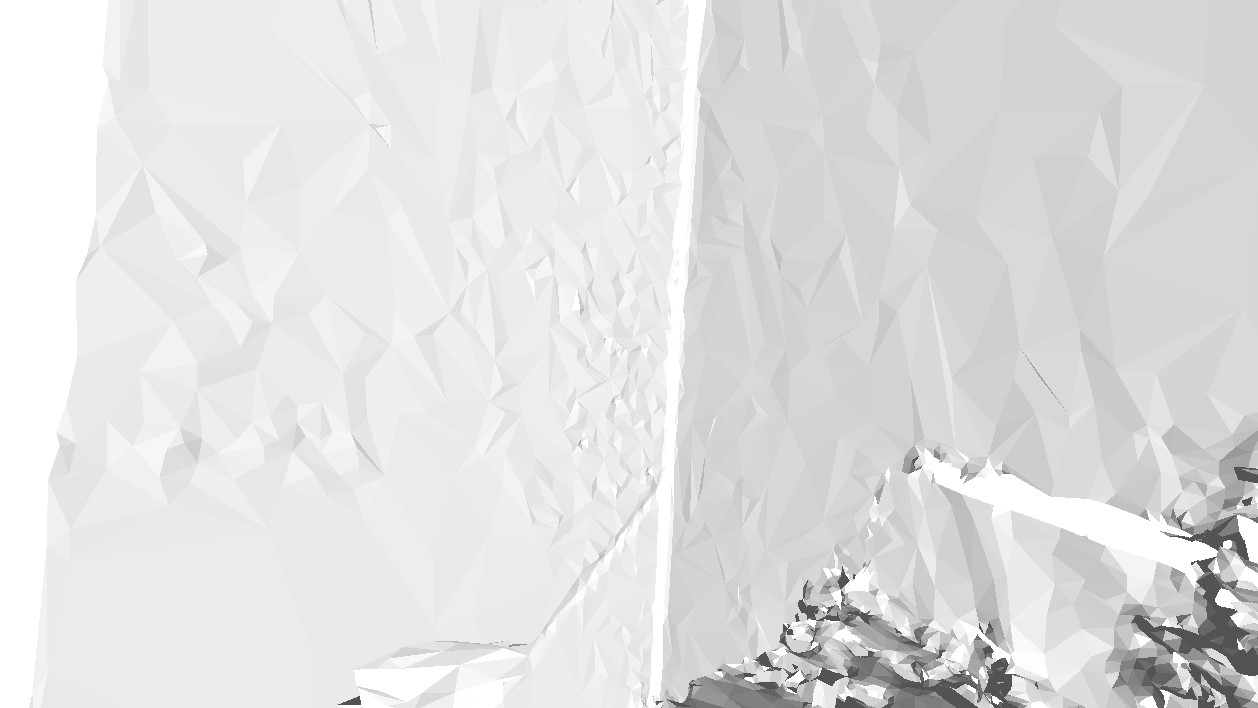
\includegraphics
		[width=0.8\columnwidth]{smooth}\caption{Simplification with smoothing}\label{smooth}\end{subfigure}\\
	\begin{subfigure}{1\textwidth}\centering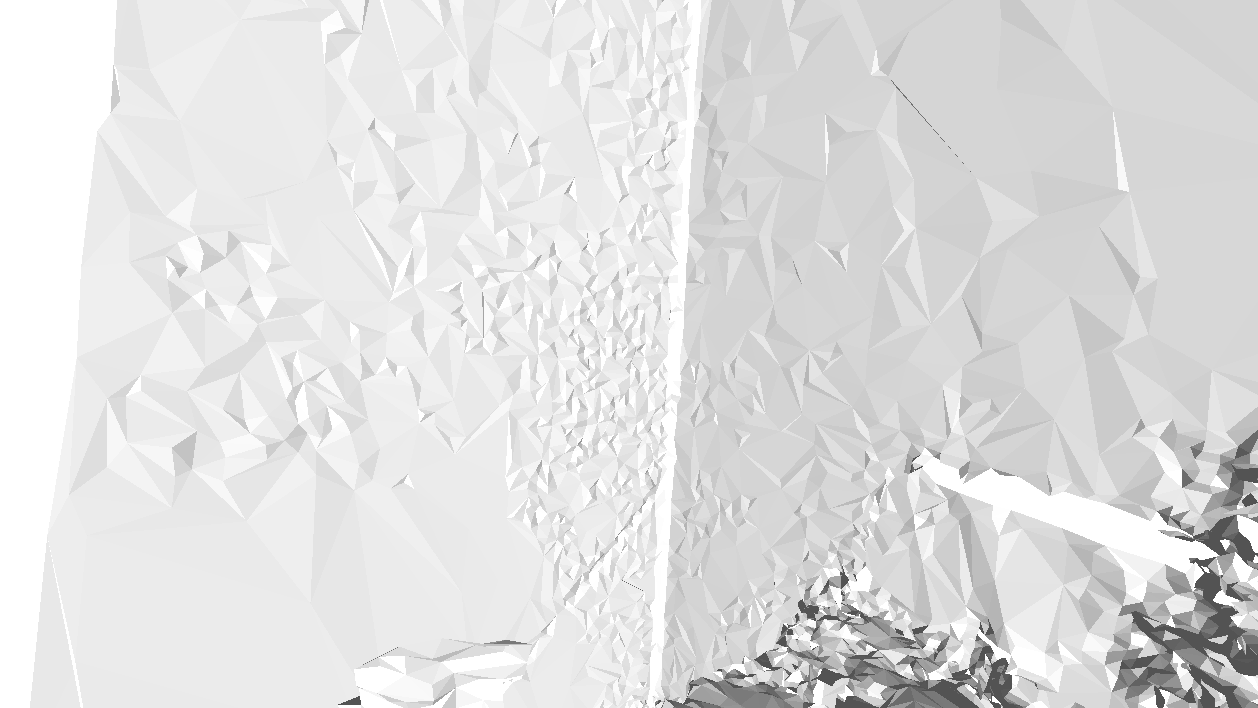
\includegraphics
		[width=0.8\columnwidth]{non_smooth}\caption{Simplification without smoothing}\label{non_smooth}\end{subfigure}
	\end{tabular}
	\caption{Comparision of the smoothing effect for 85\% simplification.}
  	\label{tab:smoothing_effect}
  	\end{center}
	\end{table}
\end{center}

\begin{table}[h!]
\centering
\begin{tabular}{ |c|c|c| } 
 \hline
 Iterations & Lambda & Mu\\
 \hline
 7 & 0.5 & -0.67\\ 
 \hline
\end{tabular}
\caption{Taubin algorithm parameters.}
\end{table}
\newpage
The simplification was ran on the mesh with 396277 faces and 208825 vertices. The mesh was reduced to 50009 faces and 29347 vertices. In Table \ref{fig:time_speedup} it can be seen that the speedup compared with the single core is around 1.6. Additionally, in the Table \ref{tab:smoothing_effect} shows that planar surfaces look better after simplification with smoothing.

\begin{table}[h!]
\centering
\begin{tabular}{ |c|c| } 
 \hline
 Time with smoothing & Time without smoothing\\
 \hline
 27.73 s & 43.06 s\\ 
 \hline
\end{tabular}
\caption{Taubin algorithm parameters.}
\label{fig:time_speedup}
\end{table}

\begin{figure}[h!]
  \begin{center}
    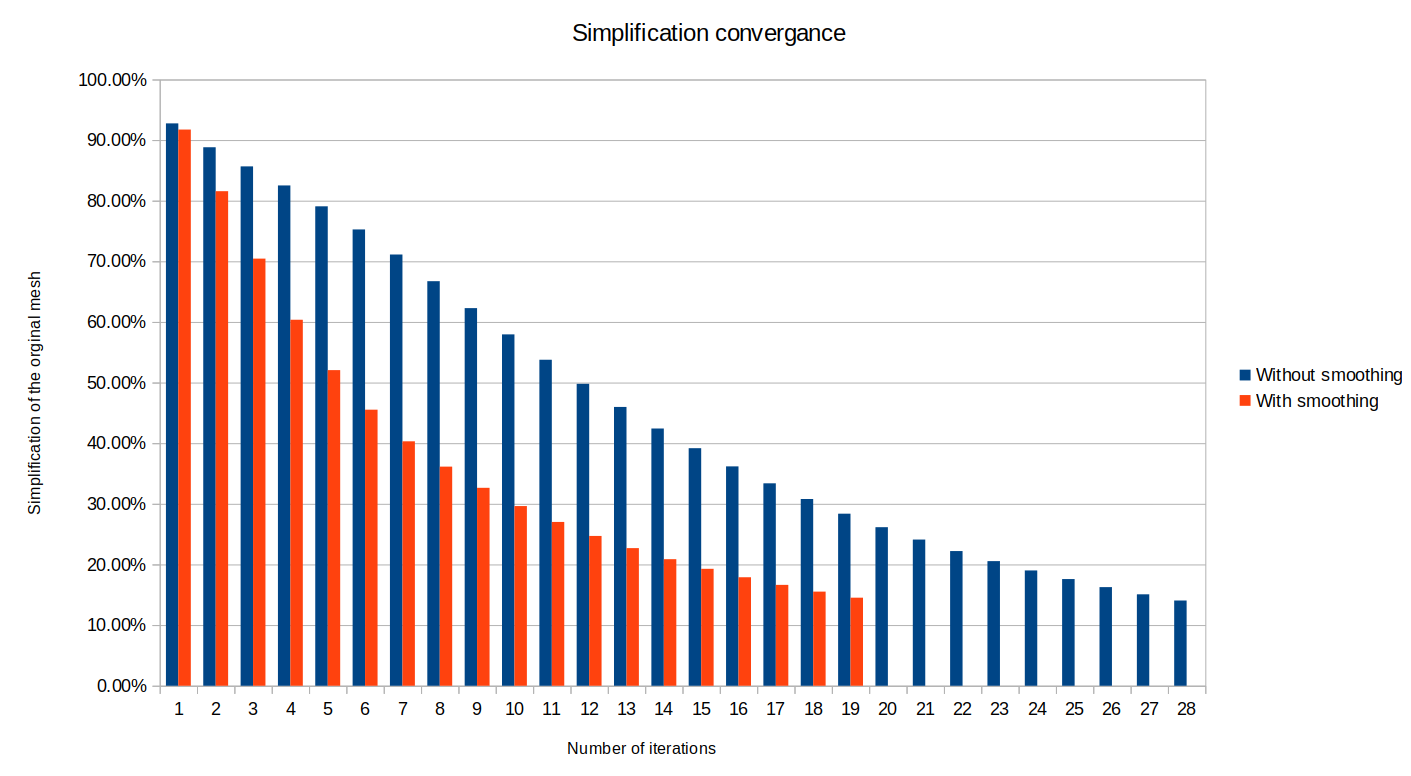
\includegraphics[width=16cm]{convergance}
    \caption{Convergance to 15\% of the original mesh.}
    \label{fig:convergance}
  \end{center}
\end{figure}

Figure \ref{fig:convergance} shows comparison of the algorithm execution with and without smoothing. In the case with smoothing, the convergance takes only 19 full iterations, whereas, for a regular version it takes 28. It means that with a small overhead, the complexity of Taubin's algorithm is linear $O(n)$ in the number of vertices \cite{taubin95}, a better quality of the simplified mesh and additional speedup can be obtained.

\newpage
\section{Summary of the Algorithm}

\begin{enumerate}
\item Smooth mesh using Taubin's algorithm (optional).
\item Cluster the mesh:
\begin{enumerate}
\item Split the mesh according to number of selected clusters; for example 2x2x2=8.
\item Add a task for each cluster to the queue.
\end{enumerate}
\item Wait for all threads from the thread-pool to finish processing simplification algorithm [QSlim] ran on all clusters. Each thread does:
\begin{enumerate}
\item Build the heap with edges.
\item Decimate edges till reaching the threshold level.
\end{enumerate}
\item Update the mesh structure:
\begin{enumerate}
\item Remove faces flagged as invalid\footnote{Removed faces and vertices are flagged as invalid due to the parallel nature of the algorithm and not thread-safe graph structure used in the implementation. Once the parallel processing is done, faces and vertices can be safely deleted from the graph.}.
\item Reset properties for each remaining face and vertex.
\end{enumerate}
\item Repeat from the second step till convergence.
\end{enumerate}

As it is shown above, the parallel algorithm nicely wraps Garland's algorithm in the third step. Procedure from the second step is repeated till either reduction level is reached, or the number of iterations is exceeded. To achieve a simplification focused on planar surfaces the adaptive threshold level is used. The third step is terminated for a given thread if the cost level is higher than the threshold.

\newpage
\section{Comparison to Commercially Available Products}

Most of commercially available algorithms use only geometry to generate an approximation of a mesh. Libraries like OpenMesh do not provide an API to use all attributes of a vertex. Moreover, increasing the number of constraints does not help. The problem is not solved jointly like in the case of this work. Additionally, those algorithms simplify a mesh globally, which introduces almost even decimation for all surfaces. Below is shown a comparison between this method and several different approaches available commercially. The benchmark was to reduce the original mesh by 85\%.

\begin{figure}[H]
  \begin{center}
    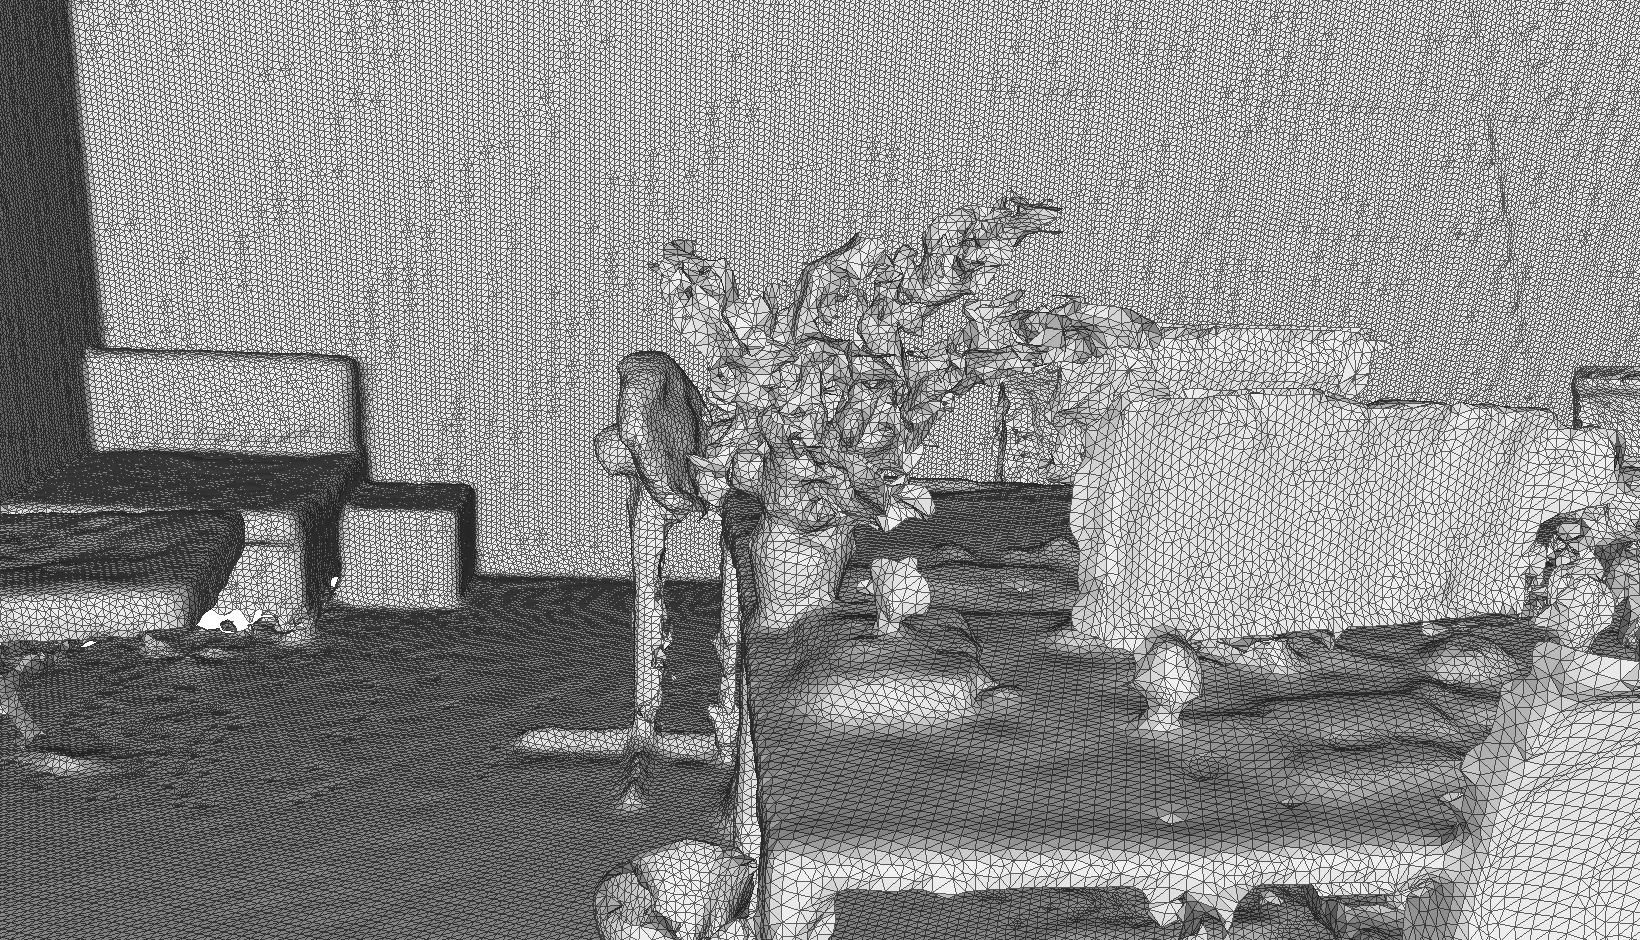
\includegraphics[width=16cm]{original}
    \caption{The original mesh.}
    \label{fig:original}
  \end{center}
\end{figure}

Figure \ref{fig:original} shows the original mesh with evenly distributed faces. The amount of faces used for the wall is unnecessary. Therefore, a successful simplification can be applied to this surface.

\begin{figure}[H]
  \begin{center}
    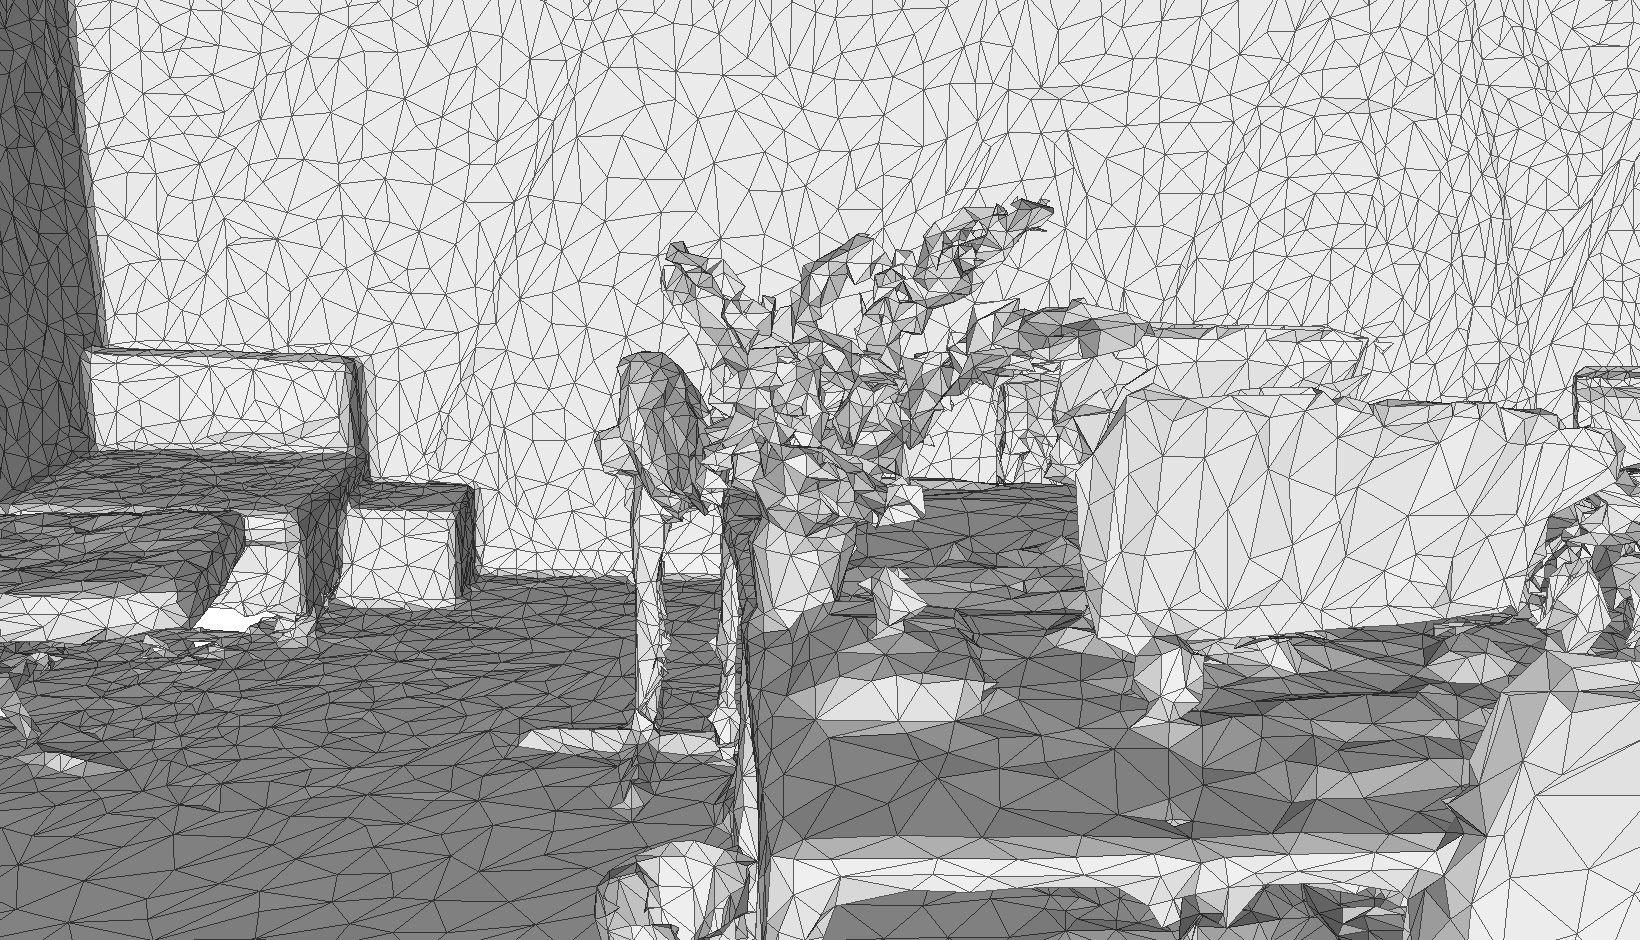
\includegraphics[width=16cm]{fast_collapse}
    \caption{Fast-Quadric-Mesh-Simplification algorithm.}
    \label{fig:fast_collapse}
  \end{center}
\end{figure}

Figure \ref{fig:fast_collapse} shows Fast-Quadric-Mesh-Simplification algorithm by Sven Forstmann, which is \href{https://github.com/sp4cerat/Fast-Quadric-Mesh-Simplification}{a Github implementation} of memory efficient and very fast edge collapse mesh simplification method. According to the creator it is around 4 times faster than the Meshlab version. Figure \ref{fig:fast_collapse} shows the result where it can be seen that all surfaces are decimated evenly. Moreover, the algorithm is based only on vertex iteration with adaptive thresholding without building a heap of edges.

\begin{figure}[H]
  \begin{center}
    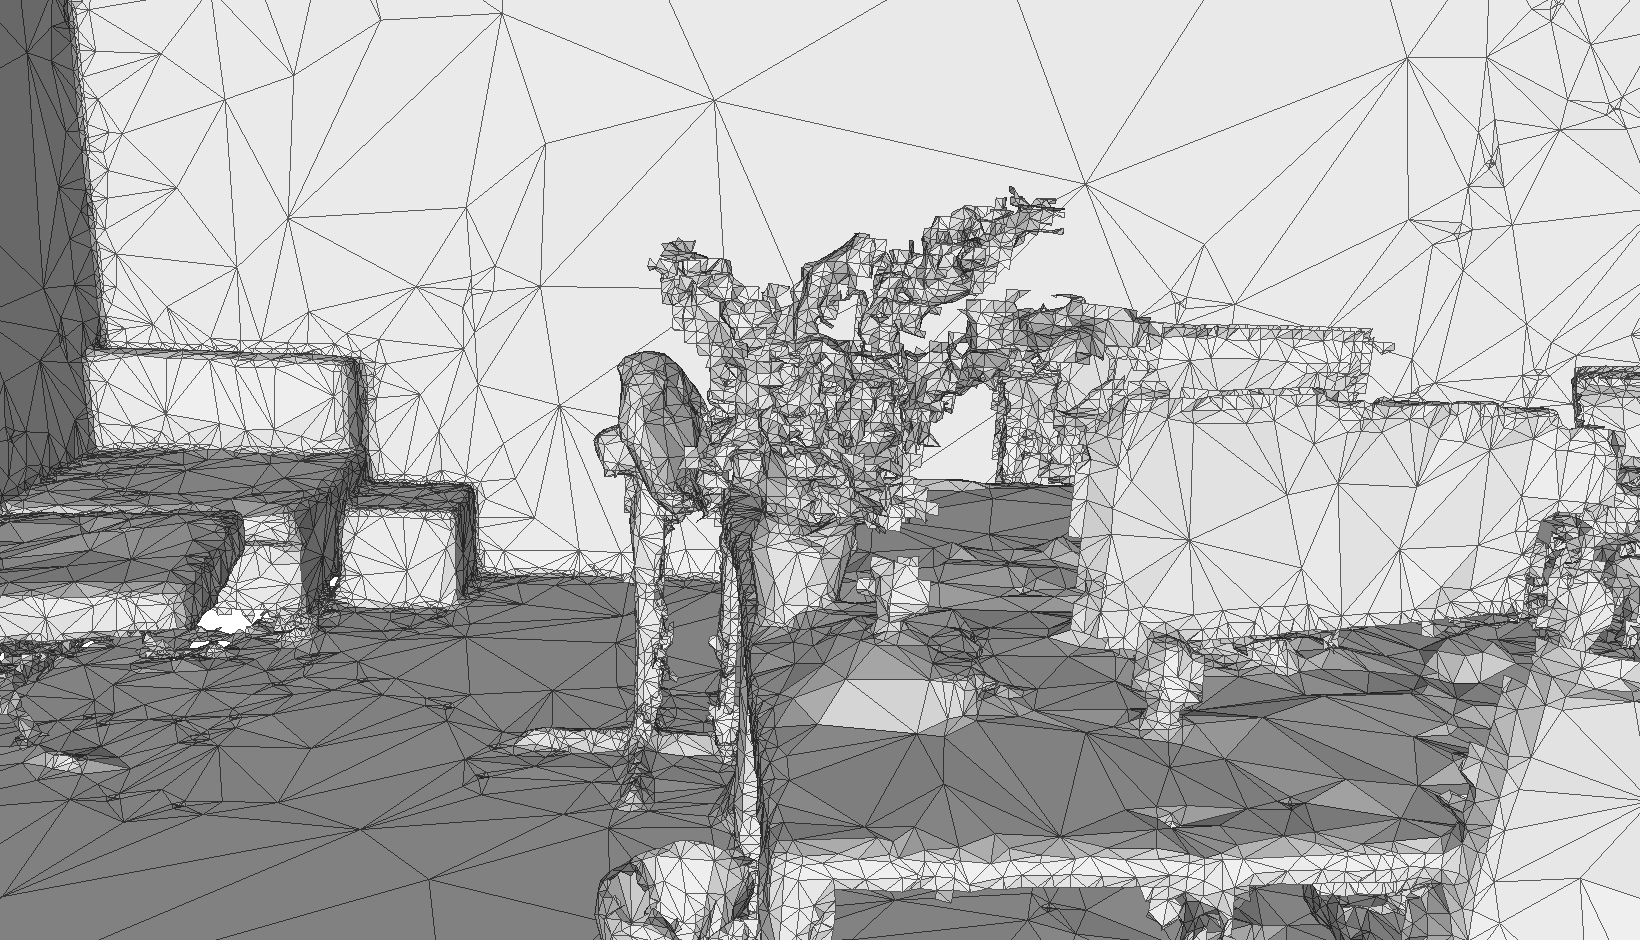
\includegraphics[width=16cm]{open_mesh}
    \caption{OpenMesh with geometry and normals.}
    \label{fig:open_mesh}
  \end{center}
\end{figure}

Figure \ref{fig:open_mesh} shows the usage of OpenMesh library, where the decimation was done using geometry and normals. Because of that, border edges were not touched. In this case, borders can produce topology errors in the approximation, like spiky edges. Border preserving is mostly visible on the plant structure or the monitors edges. This method gives the poorest result, however, it is almost as fast as Fast-Quadric-Mesh-Simplification.

\begin{figure}[H]
  \begin{center}
    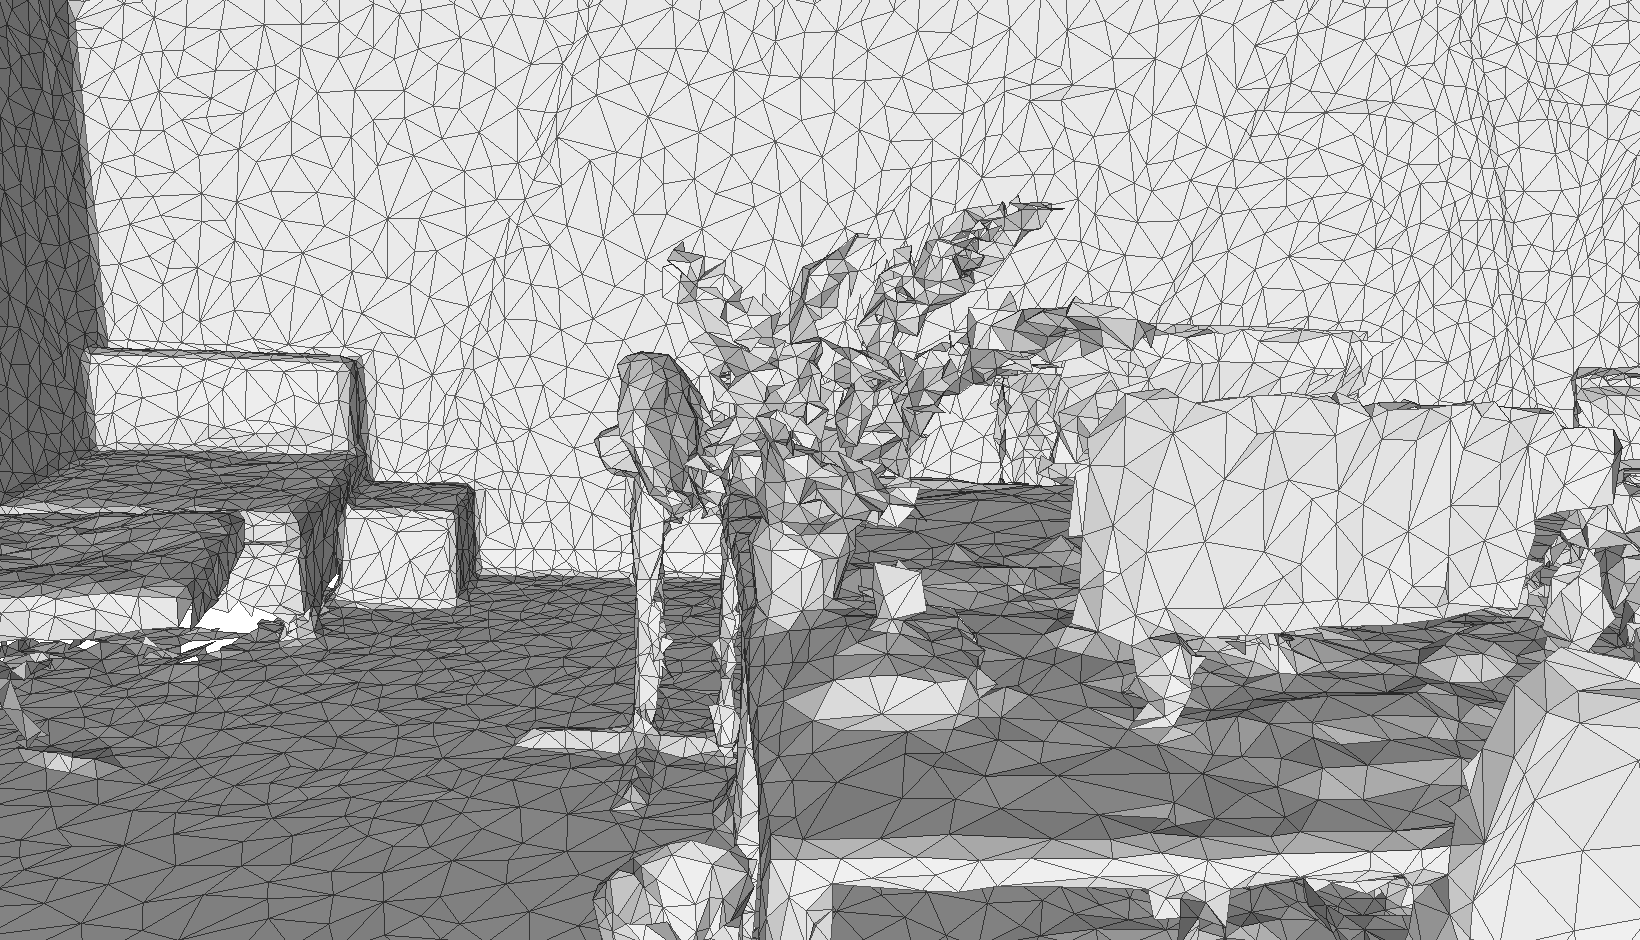
\includegraphics[width=16cm]{mesh_lab}
    \caption{MeshLab version of simplification.}
    \label{fig:mesh_lab}
  \end{center}
\end{figure}

As it can be seen in Figure \ref{fig:mesh_lab} the approximation is very similar to Figure \ref{fig:fast_collapse}. However, the MeshLab version is slower than Fast-Quadric-Mesh-Simplification algorithm.

\begin{figure}[H]
  \begin{center}
    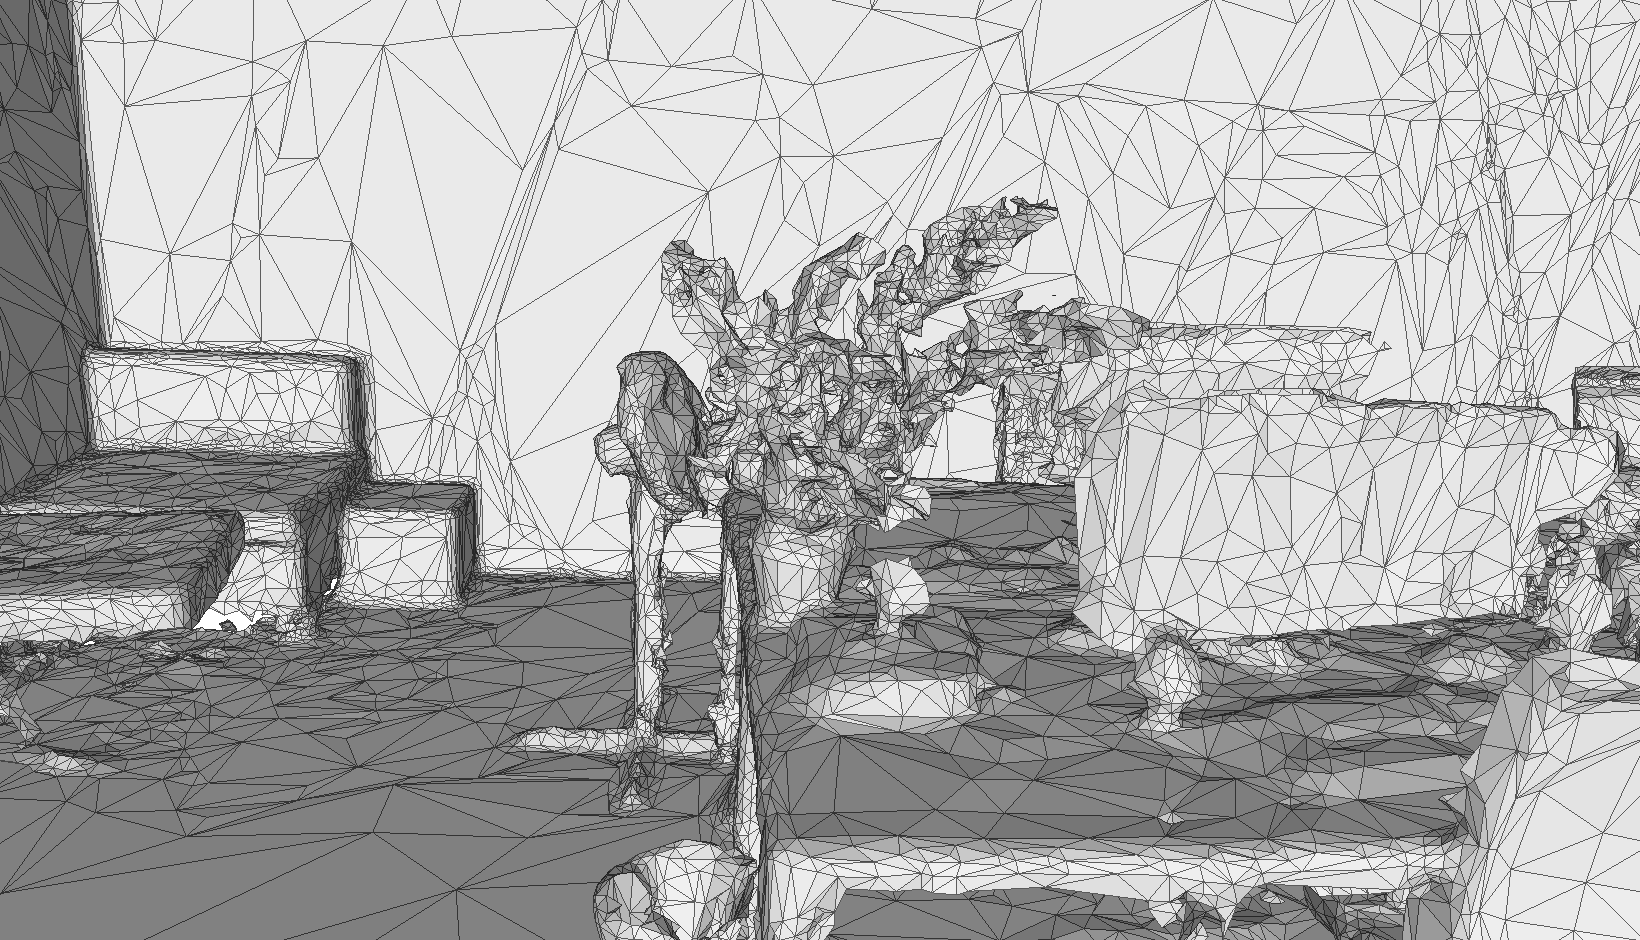
\includegraphics[width=16cm]{my_3}
    \caption{Parallel QSlim with adaptive thresholding algorithm using only geometry.}
    \label{fig:my_3}
  \end{center}
\end{figure}

Figure \ref{fig:my_3} shows approximation produced by the version of the algorithm elaborated in chapter 4. The complex shapes are preserved much better than in all previous versions. However, there is still room for even more aggressive decimation of planar surfaces. To achieve it, we need to use more attributes in our joint optimization.

\begin{figure}[H]
  \begin{center}
    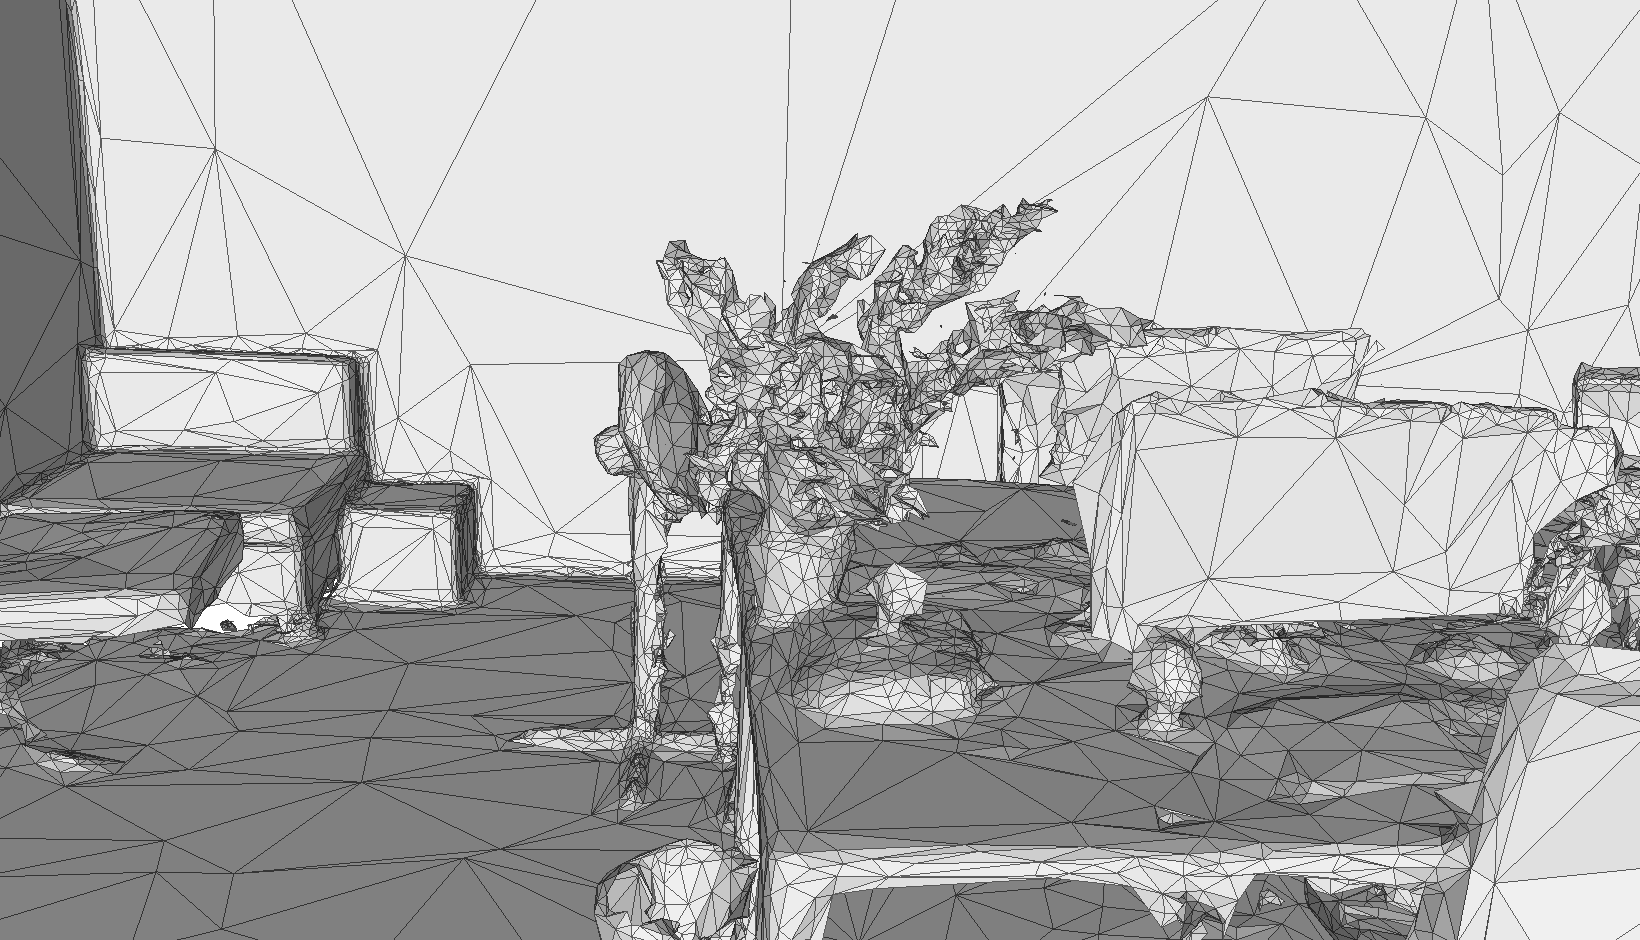
\includegraphics[width=16cm]{my_9}
    \caption{Parallel QSlim with adaptive thresholding algorithm using geometry, color and normals.}
    \label{fig:my_9}
  \end{center}
\end{figure}

Figure \ref{fig:my_9} shows the best approximation under the constrain of decimating most of the planar surface. All complex shapes are almost completely preserved from the original mesh. The faces which describe the wall are as big as possible. Moreover, iterative nature of the algorithm, allows to level small surface elevation changes. For instance, the interior part of the pouf near the wall. In Figure \ref{fig:my_3} it can be seen that the noise and level changes, meaning high quadric error, prevents this region from being simplified. In the version with all attributes $[geometry, normal, color]$, the interior part is nicely leveled.

\begin{figure}[H]
  \begin{center}
    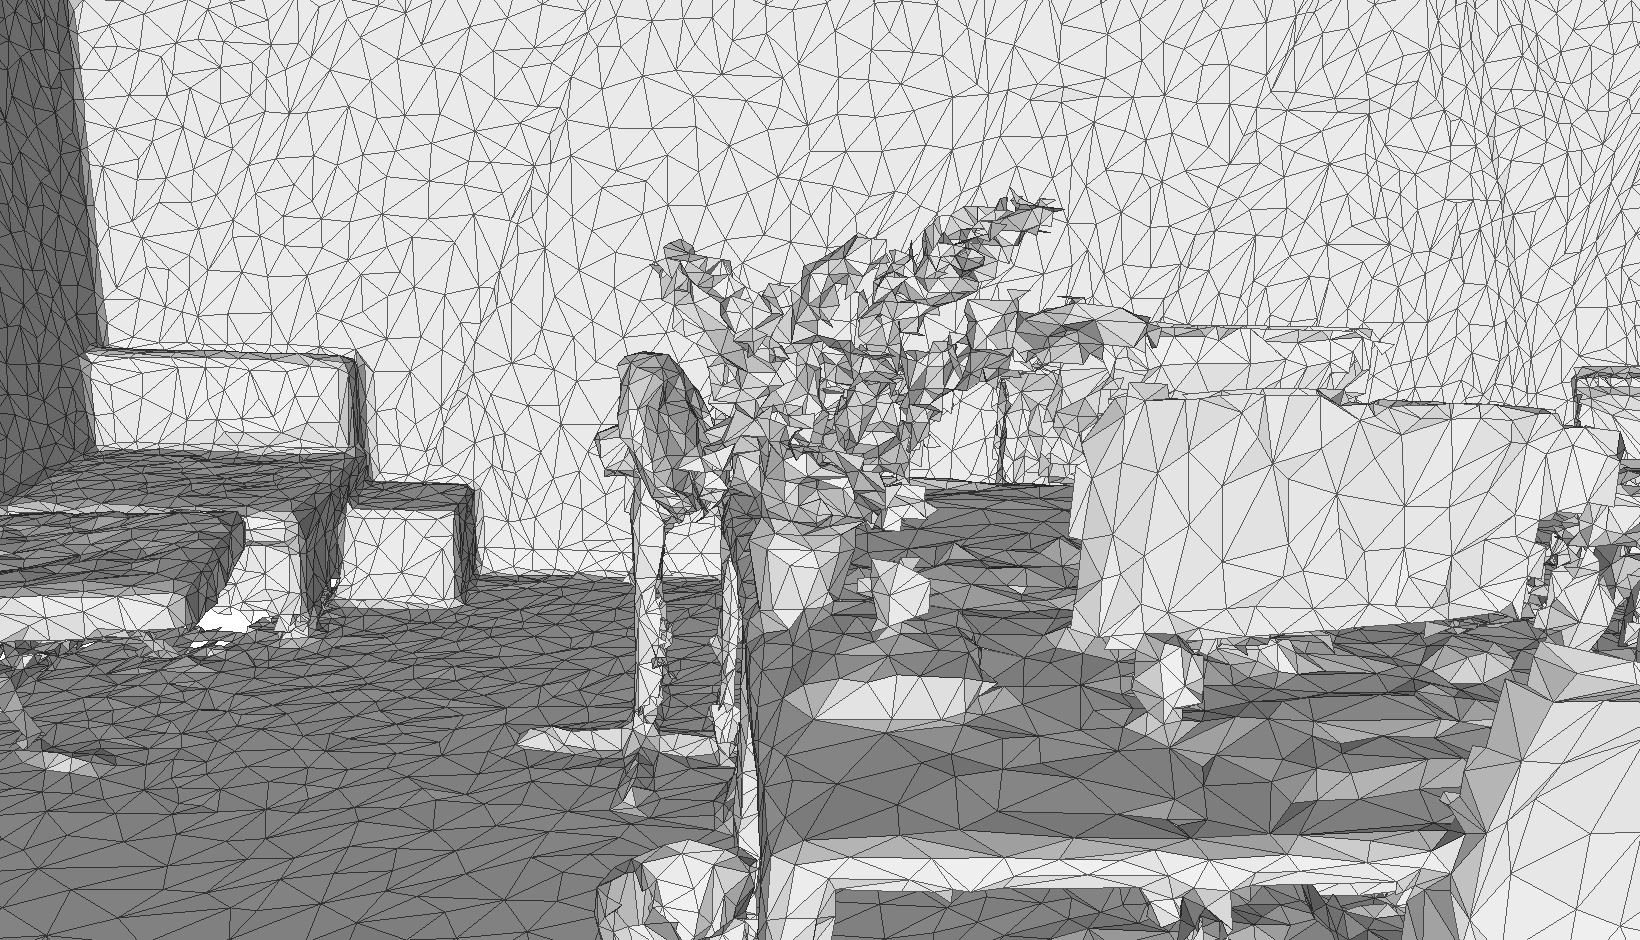
\includegraphics[width=16cm]{rapid_compact}
    \caption{RapidCompact version of simplification.}
    \label{fig:rapid_compact}
  \end{center}
\end{figure}

For completeness, a commercial version of simplification algorithm was used. The algorithm was provided by the company RapidCompact. Figure \ref{fig:rapid_compact} shows that the result is almost exactly the same, like in the case of the MeshLab and Fast-Quadric-Mesh-Simplification algorithm.
